\documentclass[useAMS, usenatbib, preprint, 12pt]{aastex}
% \documentclass[a4paper,fleqn,usenatbib,useAMS]{mnras}
\usepackage{cite, natbib}
\usepackage{float}
\usepackage{epsfig}
\usepackage{cases}
\usepackage[section]{placeins}
\usepackage{graphicx, subfigure}
\usepackage{color}
\usepackage{bm}

\newcommand{\ie}{{\it i.e.}}
\newcommand{\eg}{{\it e.g.}}
\newcommand{\etal}{{\it et al.}}

\newcommand{\kepler}{{\it Kepler}}
\newcommand{\corot}{{\it CoRoT}}
\newcommand{\Ktwo}{{\it K2}}
\newcommand{\ktwo}{\Ktwo}
\newcommand{\TESS}{{\it TESS}}
\newcommand{\tess}{{\it TESS}}
\newcommand{\LSST}{{\it LSST}}
\newcommand{\lsst}{{\it LSST}}
\newcommand{\Wfirst}{{\it WFIRST}}
\newcommand{\wfirst}{{\it WFIRST}}
\newcommand{\SDSS}{{\it SDSS}}
\newcommand{\PLATO}{{\it PLATO}}
\newcommand{\plato}{{\it PLATO}}
\newcommand{\Gaia}{{\it Gaia}}
\newcommand{\gaia}{{\it Gaia}}
\newcommand{\panstarrs}{{\it PanSTARRS}}

\newcommand{\Teff}{$T_{\mathrm{eff}}$}
\newcommand{\teff}{$T_{\mathrm{eff}}$}
\newcommand{\FeH}{[Fe/H]}
\newcommand{\feh}{[Fe/H]}
\newcommand{\prot}{$P_{\mathrm{rot}}$}
\newcommand{\pmega}{$\bar{\omega}$}
\newcommand{\mj}{$m_j$}
\newcommand{\mh}{$m_h$}
\newcommand{\mk}{$m_k$}
\newcommand{\mx}{$m_x$}
\newcommand{\logg}{log(g)}
\newcommand{\dnu}{$\Delta \nu$}
\newcommand{\numax}{$\nu_{\mathrm{max}}$}

\newcommand{\amnh}{1}
\newcommand{\cca}{2}
\newcommand{\columbia}{3}
\newcommand{\florida}{4}
\newcommand{\riverside}{5}

\newcommand{\sd}{{\tt stardate}}
\newcommand{\MS}{main sequence}
\newcommand{\ms}{main sequence}
\newcommand{\Ms}{Main sequence}
\newcommand{\gcolor}{$G_{BP} - G_{RP}$}
\newcommand{\fhat}{$\hat{F}$}
\newcommand{\cbv}{$C_{B-V}$}

\newcommand{\racomment}[1]{{\color{red}#1}}

\begin{document}

% \title{Inferring stellar ages by combining isochrone fitting with
% gyrochronology}
\title{A new age-dating model for cool main sequence stars that combines
stellar evolution models with gyrochronology}
% \title{A new age-dating model for cool main sequence stars that combines
% stellar evolution models with gyrochronology}

\author{%
    Ruth Angus\altaffilmark{\amnh, }\altaffilmark{\cca, }\altaffilmark{\columbia},
    Timothy D. Morton\altaffilmark{\florida, }\altaffilmark{\cca, },
    Stephen Kane\altaffilmark{\riverside},
   \etal\ (TBD)
}

\altaffiltext{\amnh}{American Museum of Natural History, Central Park West,
Manhattan, NY}
\altaffiltext{\cca}{Center for Computational Astrophysics, Flatiron Institute,
162 5th Avenue, Manhattan, NY}
\altaffiltext{\columbia}{Department of Astronomy, Columbia
University, NY, NY}
\altaffiltext{\florida}{Department of Astronomy, University of Florida,
Gainesville, FL}
\altaffiltext{\riverside}{Department of Physics and Astronomy, UC Riverside,
Riverside, CA}

\begin{abstract}
    We present a new technique for inferring stellar ages that combines two
different established age-dating methods: gyrochronology and isochrone
fitting.
This method provides ages with 20\% precision across the MS and subgiant
branch.
Gyrochronology and isochrone fitting are independent age-dating methods, each
capable of providing extremely precise ages in certain areas of the
Hertzsprung-Russell diagram.
Combined, they can be applied to a much broader range of stellar masses and
evolutionary stages and can provide ages that are more precise and accurate
than either method in isolation.
Rotation periods supply precise ages for cool stars on the main sequence via
gyrochronology and isochrone fitting provides precise ages near main sequence
turn off.
In this investigation, we demonstrate that the observables of main sequence
stars used to trace core hydrogen burning and stellar evolution on the
Hertzprung-Russell diagram (\teff, \feh, \logg, parallax, apparent magnitude
and photometric colors) can be combined with \kepler\ rotation periods, in a
Bayesian framework, to infer precise stellar ages from both isochrone fitting
and gyrochronology simultaneously.
We show that incorporating rotation periods into stellar evolution models
significantly improves the precision of inferred ages on the main sequence.
However, since ages predicted with gyrochronology on the main sequence are, in
general, much more precise than isochronal ages, care must be taken to ensure
the gyrochronology relation being used is accurate.
The goal of this study is to explore the power of combining two independent
dating methods, not to recalibrate or improve upon existing gyrochronology
models.
However, only a slight modification to our algorithm would be required to
perform a calibration and, since the code is modular, an updated
gyrochronology model could easily replace the one used here in future.
This publication is accompanied by open source code ({\it Python} package,
\sd), for inferring stellar ages for cool main sequence stars and subgiants
from rotation periods, spectroscopic parameters and/or apparent magnitudes and
parallaxes.

\end{abstract}

% \label{section:intro}
% Motivation and context
%-----------------------------------------------------------------------------
%   - The need for better stellar ages.
%   - Why are MS ages harder than red giant ages?
%   - Introduce gyrochronology
%   - How does gyrochronology work?
%   - Theoretical vs empirical gyro models
%   - Motivation for improvements to gyrochronology relations
%   - Describe the project presented here.
%   - Sum up
%   - Paper outline
\section{Introduction}
\label{section:intro}

% Motivation and context
%-----------------------

%   - The need for better stellar ages.
The formation and evolution of the Milky Way (MW) and the planetary systems
within it are two topics of significant interest in astronomy today.
Both of these fields require precise and accurate ages for tens to hundreds of
thousands of stars.
% Precise ages of red giant stars, some calculated from asteroseismology, some
% from spectroscopy, some from physical models and some from machine learning
% methods have recently been used to explore the age distributions of stellar
% populations in the MW \citep[\eg][]{ness2015, stello2017, das2018,
% sanders2018}.
% Red giants are highly luminous and can be observed to great distances, thus
% providing age information on the scale of tens of kilo-parsecs.
% Main sequence (MS) stars on the other hand, although fainter, are more
% numerous and so their ages may provide new insights into the formation and
% evolution of the Solar neighborhood.
% MS star ages are also of great interest for studying the formation and
% evolution of planetary systems.
% Almost all exoplanets discovered to date orbit MS stars and it is therefore
% {\it MS star} ages that are needed to study planet evolution.
% Unfortunately, the very property that makes MS stars good hosts for habitable
% planets also makes them difficult to date: they do not change substantially
% over time.
% There are several properties of giant stars that make them easier to date than
% MS stars.
% One property is that their acoustic oscillations have long periods of hours to
% days and large amplitudes, so they can be detected and resolved using the
% \kepler\ spacecraft's long cadence mode.
% The acoustic modes of MS stars, on the other hand, have typical periods of
% five minutes, which are unresolvable in \kepler's long cadence mode (thirty
% minutes between observations).
% The large numbers of giants with asteroseismic ages \citep[\eg][]{huber2010,
% yu2016, stello2017, yu2018, de_assis_peralta2018} provides a large training
% set for machine learning methods.
% In addition the ages of red giants are strongly correlated with their masses,
% so if mass can be measured (from the spectrum, for example), so can age
% \citep{ness2015}.
% Age is the most elusive fundamental stellar property and is extremely
% difficult to measure for field stars -- especially cool stars on the MS.
% However, a time axis is essential for studying the evolution and formation of
% any astronomical object, from a planetary system to the Milky Way itself, so
% improvements in stellar age-dating methods would have a wide-reaching impact
% across astronomy.
% For example, in the field of exoplanets the ages of planet hosting stars could
% be used to explore the dynamical and architectural evolution of planetary
% systems.
% % The typical timescales for planetary system stability could be inferred,
% % leading to implications for the fates of planetary systems in the Milky Way
% % including our own.
% New stellar ages would also benefit galactic archaeologists and could resolve
% the mystery behind the formation of the galactic thin disk.
% {\bf The need for more precise and accurate stellar ages is virtually
% universal within astronomy.}

The difficulty of age-dating is particularly acute for low mass (GKM) stars on
the MS: precisely those that comprise the majority of known planet hosts.
Using conventional dating methods, uncertainties on the ages of these stars
can be as large as the age of the Universe, in other words they are completely
unconstrained.
% , and
% ages precise to within 50\% are considered `ultra-precise'
% \citep{soderblom2010}.
The stars eligible for {\it truly} precise age-dating, where age uncertainties
can be as low as 10\%, are those in nearby open clusters, those with
observable acoustic oscillations (asteroseismic stars), those just turning off
the MS, and the Sun
\citep[see][for a review of stellar ages]{soderblom2010}.
There are only a few tens of cool, MS stars with precise ages that are
suitable for exoplanet population studies, however {\it tens-of-thousands} of
precise ages are needed to study the evolution of planetary systems
\citep[\eg][]{petigura2013, foreman-mackey2014, veras2015, burke2015}.
The number of planets detected in open clusters, therefore with precise ages,
is growing, however there are still only a couple of dozen of these discovered
so far and the total number of detectable planets in clusters is unlikely to
reach statistical numbers in the near future, if ever.
In order to study the evolution of planetary systems, a significant number of
precise ages for cool MS {\it field} stars are needed.
Neither cluster stars nor asteroseismic stars can currently provide the
numbers required for exoplanet population studies: age-dating methods for cool
MS field stars {\it must} be improved before the evolution of planets can be
explored.

% Planetary system studies are one example of an astronomical field that would
% greatly benefit from a large stellar age catalog.
% Another notable field that requires large numbers of stellar ages is galactic
% archaeology.
% Machine learning methods have significantly improved age-dating for field red
% giant stars recently, and large-scale catalogs of precise giant ages have lead
% to dramatic breakthroughs in galactic archaeology \citep[\eg][]{ness2015,
% das2018, sanders2018}, but these methods are not yet applicable to MS stars,
% yet MS stars are more numerous than red giants and their ages could
% revolutionize galactic archaeology.
% The largest catalog of precise ages for field {\it MS} stars currently
% available is the short-cadence Kepler asteroseismic catalog of 500 stars
% \citep{chaplin2014}.
% However, few of these stars are truly on the MS (most are on the subgiant
% branch) and even fewer are cool -- most being A, F and G types.
% There is currently {\it no} large catalog of stellar ages for field MS stars,
% and there is unlikely to be one until after the launch of {\it PLATO} and the
% release of a large catalog of asteroseismic properties.

%   - Why are MS ages harder than red giant ages?
% Unlike red giants, the masses of MS stars are not strongly correlated with
% age, so mass cannot be used as an age proxy.
The spectra and colors of MS stars do not contain a significant amount of age
information because they do not change rapidly.
This is represented in the spacing of isochrones on a Hertsprung-Russell (HR)
or color-magnitude diagram (CMD).
On the MS, isochrones are tightly spaced and, even with very precise
measurements of effective temperature and luminosity, the position of a MS
star on the HR diagram may be consistent with range of isochrones spanning
several billion years.
At main sequence turn-off however, isochrones are spread further apart, so
that sufficiently precisely measured temperatures and luminosities may yield
ages that are extremely precise.
% Typical age uncertainties of dwarfs.
The classical method for measuring stellar ages is called isochrone placement,
or isochrone fitting, where surface gravity changes resulting from fusion in
the core (usually observed via luminosity, $L$, and effective temperature,
\teff, or absolute magnitude and colour) are compared with a set of models
that trace stellar evolution across the Hertzprung-Russell, or color-magnitude
diagram (CMD).
Surface gravity changes have been thoroughly mapped with physical models, and
can be used to calculate relatively accurate (but not necessarily precise)
ages, barring some small, $\sim$10\% variations between different models
\citep[\eg][]{yi2001, dotter2008, dotter2016}.
Isochronal ages {\it can} be precise for stars turning off the MS, because the
rate of change in brightness and temperature is large during this phase of
stellar evolution.
However, on the MS itself, there is little differentiation between stars of
different ages in the $L$ and \teff\ plane, so ages tend to be very imprecise.
The method of inferring a star's age from its rotation period, called
`gyrochronology', is much better suited for measuring ages on the MS because
MS, stars spin down relatively rapidly.

%   - How does gyrochronology work?
Magnetic braking in MS stars was first observed by \citet{skumanich1972} who,
studying young clusters and the Sun, found that the rotation periods of
Solar-type stars decay with the square-root of time.
It has since been established that the rotation period of a star depends, to
first order, only on its age and mass \citep[\eg][]{barnes2003}.
This means that by measuring a star's rotation period and a suitable mass
proxy (B-V color is commonly used), one can determine its age.
The convenient characteristic of stars that allows their ages to be inferred
from their {\it current} rotation periods and independently of their
primordial ones, comes from the steep dependence of spin-down rate on rotation
period \citep{kawaler1989}.
% Observations of young clusters indicate that stellar angular momentum loss
% rate is proportional to the cube of the angular velocity.
This means that a star spinning with high angular velocity will experience a
much greater angular momentum loss rate than a slowly spinning star.
For this reason, no matter the initial rotation period of a Sun-like star,
after around the age of the Hyades (500-700 million years) stellar rotation
periods appear to converge onto a tight sequence \citep{irwin2009}.
After this time, the age of a star can be inferred, to first order, from its
mass and rotation period alone and this is the principle behind gyrochronology.

% % Explain the project (add more detail here.)
% In this work we present and test a new age-dating model that combines stellar
% evolution models with an empirical gyrochronology model in a Bayesian
% framework.
% This approach has an advantage over either isochrone fitting or gyrochronology
% alone since the addition of age-relevant information will always improve
% stellar age estimates, unless the models are wrong.

%   - Theoretical vs empirical gyro models
The relation between age, rotation period and mass has been studied in detail,
and several different models have been developed to capture the rotational
evolution of Sun-like stars.
Some of these models are theoretical and based on physical processes; modeling
angular momentum loss as a function of the stellar properties as well as the
properties of the magnetic field and stellar wind \citep{kawaler1988,
kawaler1989, vansaders2013, matt2015, vansaders2016}.
Other models are empirical and capture the behavior of stars from a purely
observational standpoint, using simple functional forms that can reproduce the
data \citep{barnes2003, barnes2007, mamajek2008, angus2015}.
Both types of model, theoretical and empirical, must be calibrated using
observations.
% Even the theoretical models are highly sensitive to some stellar properties
% that are not measurable: mass-loss rate and magnetic field geometry, for
% example.
Old calibrators are especially important because new evidence suggests that
rotational evolution goes through a transition at old age or, more
specifically, at a large Rossby number, $Ro$ (the ratio of rotation period to
the convective overturn timescale).
For example, old \kepler\ asteroseismic stars rotate more rapidly than
expected given their age \citep[\eg][]{angus2015, vansaders2016}.
A new physically motivated gyrochronology model, capable of reproducing these
data, was recently introduced \citep{vansaders2016}.
It relaxes magnetic breaking at a critical Rossby number of around the Solar
value, 2.1.
This model predicts that, after stellar rotation periods lengthen enough to
move stars cross this $Ro$ threshold, stars stop spinning down and maintain a
constant rotation period from then until they evolve off the MS.
The implication is that the ages of stars with $Ro >$ 2.1 cannot be measured
from their rotation periods.
% Despite recent advances in rotation-dating, such as the new $Ro$ transition
% models \citep{vansaders2016, vansaders2018}, there is still substantial room
% for improvement in the gyrochronology relations.

% %   - Motivation for improvements to gyrochronology relations
% % For example, there is, as yet no {\it fully} empirical gyrochronology model
% % that includes a weakened magnetic braking law after the $Ro$ = 2.1 transition.
% Empirical models have value as they are often more flexible than physical
% models and can capture trends in the data before the physical processes at
% work are fully understood.
% In addition, no single gyrochronology relation can reproduce the rotational
% behaviour of all open clusters; the relation between rotation period, age and
% mass varies from cluster to cluster in a way that cannot be captured by
% any current model.
% Again, this is related to the issue of model flexibility.
% Finally, more stars with precisely measured old ages are needed to confidently
% calibrate gyrochronology models at old ages.
% New asteroseismic calibrators will become available from reprocessed \kepler\
% short cadence light curves, however significant numbers of suitable
% gyrochronology calibrators may not be accessible until after the European
% Space Agency's \plato\ mission is launched.

%   - Describe the project presented here.
The gyrochronology models that capture post $Ro$-threshold, rotational
evolution \citep{vansaders2016} are the current state-of-the-art in rotation
dating.
% developed and calibrated in \citet{epstein2014, vansaders2015,
% vansaders2016, vansaders2018} However, despite their superior accuracy, they
These models are expensive to compute and, just as with most isochrones and
stellar evolution tracks, are usually pre-computed over a grid of stellar
parameters, then interpolation is used to predict the age of a star.
The process of measuring a stellar age with these models is similar to
inferring an age using any set of isochrones, with the main difference being
that rotation period is an additional dimension.
Ages calculated using these models are therefore likely to be much more
precise than using rotation-free isochrones since rotation period provides an
additional anchor-point for the age of a star.
% In order to infer an age from these models, one would effectively perform
% isochrone fitting but in this case, rotation period would be added as an
% additional parameter and the ages inferred would therefore be more precise and
% accurate.
We present here a complementary method that combines isochrones with an {\it
empirical} gyrochronology model using a Bayesian framework.
The methodology is related to the models described above \citep{vansaders2016}
in that both use a combination of rotation periods and other observable
properties that track stellar evolution on the HR diagram in concert.
The main difference is that the gyrochronology model used here is an entirely
empirically calibrated one, as opposed to a physically derived one.
One major advantage of using a physically motivated gyrochronology model over
an empirically calibrated one is the ability to rely on physics to interpolate
or extrapolate over parts of parameter space with sparse data coverage.
However, rotational spin-down is a complex process that is not yet fully
understood and currently no physical model can accurately reproduce all the
data available.
For this reason, even physically motivated gyrochronology models cannot always
be used to reliably extrapolate into unexplored parameter space.
Physical models, when calibrated to data can provide insight into the physics
of stars however, if accurate and precise {\it prediction} of stellar
properties is desired, empirical models can have advantages over physical
ones.
For example, the data may reveal complex trends that cannot be reproduced with
our current understanding of the physical processes involved but may be
captured by more flexible data-driven models.
In addition, it is relatively straightforward to build an element of
stochasticity into empirical models, \ie\ to allow for and incorporate
outliers or noisy trends.
This may be particularly important for stellar spin down, which does not
always seem to behave predictably.
% For example, synchronized binaries often appear to be rapidly rotating single
% stars which do not fall on the gyrochronology sequence and are perhaps one of
% the most common cause of outliers.
% One can never be certain that the rotation period of any given star truly
% reflects its age: there is a chance that it is an outlier.
% The probability that a star is an outlier in rotation-color-age space can be
% modeled and incorporated easily into an empirical gyrochronology model.
% In a deterministic model, a star with a rotation period that misrepresents its
% age will have a precise but extremely inaccurate inferred age.
% If however, some allowance for outliers or instrinsic scatter is built into
% the models, such a star would be recognized as an outlier and would have a
% very imprecise but accurate inferred age.
% The relation between rotation period and age for M dwarfs is noisy, and a
% deterministic model would not be appropriate for these stars: it would lead to
% inaccurately predicted ages with over-optimistic precision.
% Instead, these data could be appropriately modeled with a stochastic mixture
% of broad Gaussians, or similar.
A further advantage of empirical models is that inference is more tractable:
it can be extremely fast to fit them to data.
We use a simple, empirical, deterministic gyrochronology model in this work,
which, like any other gyrochronology model, cannot yet reproduce all the
observed data.
Simple modifications could be made to this model to produce
significant improvements, for example, by including instrinsic scatter and
outliers, however we leave these improvements for a future project.
% For example, an allowance for outliers; stars with anomalously fast or slow
% rotation periods, could be build into our model.
Ultimately, the model we present here will provide a baseline against which
other gyrochronology models can be compared.

% Despite significant advances in both theoretical and empirical gyrochronology
% models, no existing model is currently able to reproduce the data.
% % theoretical models of stellar spin-down as well as new calibrations of
% % empirical models, the gyrochronology relations have not yet been finalized
% % because
% New high quality rotation periods recently measured from Kepler/K2
% observations reveal that rotational evolution is more complicated than
% previously thought, partly because the shape of the rotation-color relation is
% different and unique for each cluster \citep{meibom2011, meibom2015,
% rebull2016, douglas2016, rebull2017, douglas2017} and partly because stars
% appear to stop spinning down at old ages \citep{angus2015, vansaders2016,
% vansaders2018}.
% Theoretical models have been developed to reproduce the lack of magnetic
% braking at old ages \citep{vansaders2016, vansaders2018}, however no model has
% yet been designed to fit the individual shape of every cluster.
% In addition, the relation between rotation period, color and age appears to be
% stochastic at all ages and masses, particularly for young and low-mass
% stars.
% The gyrochronology relations could be improved in three main ways.
% Firstly,
% because stellar evolution is a noisy process that produces outliers and
% scatter, gyrochronology models could be non-deterministic.
% Secondly, the gyrochronology models could be more flexible in order to
% capture the inter-cluster variation in the shape of the rotation-color
% relations.
% Finally, new calibrators are needed to more precisely constrain rotational
% evolution at low masses and old ages.
%  % for two main reasons.
% % Firstly, the rotational evolution of stars is complex and not well understood.
% % It is difficult to reproduce the trends in the data using the known physical
% % processes acting within stellar interiors, surfaces and winds.
% % It is also challenging to come up with an empirical model that is flexible
% % enough to capture trends in the data.
% % Secondly, there is a lack of suitable calibration stars with precisely
% % measured ages, particularly at old ages.  % and low masses.
% % % These regions of parameter space are especially important because some
% % % evidence suggests that rotational evolution goes through a transition at old
% % % ages and low masses.
% % % This region of parameter space is especially important because new evidence
% % % This region of parameter space is


% Paper outline
%-----------------------------------------------------------------------------
This paper is laid out as follows.
In section \ref{section:motivation} we provide additional motivation for
combining gyrochronology and isochrone fitting by providing examples based
on information theory.
In section \ref{section:method} we describe our new age-dating model and its
implementation, in section \ref{section:results} we test this model on
simulated stars, cluster stars and asteroseismic stars, and in section
\ref{section:discussion} we discuss the implications of these tests and future
pathways for development.
Throughout this paper we use the term {\it `observables'} to refer to the
following observed properties of a star, \teff, \logg, observed bulk
metallicity ($[\hat{\mathrm{Fe/H}}]$), parallax ($\bar{\omega}$), photometric
colors in different passbands ($\bf{m_x}$) and rotation period
($P_{\mathrm{rot}}$).
The term {\it `parameters'} refers to the physical properties of that star:
age ($A$), mass ($M$), true bulk metallicity (\feh), distance ($D$) and V-band
extinction ($A_V$).
These are the properties that generate the observables.


\section{Combining isochrone fitting with Gyrochronology: Motivation}
\label{section:motivation}

In order to demonstrate why a combination of gyrochronology and isochrone
fitting can provide more precise ages than either method used in isolation, we
calculated the information provided by each method for a range of stellar
masses, ages and evolutionary stages.

According to observations of cluster stars and the Sun, the decrease in
rotation period with time is roughly proportional to the inverse square root
of age, $\frac{dP_{\mathrm{rot}}}{dt} \propto \mathrm{Age}^{-n}$, where
n$\sim$0.5.
This corresponds to a large rate of change relative to typical rotation
period measurement uncertainties.
For example, the Sun's rotation period is currently decreasing at a rate of
around 3 days per billion years \citep[unless it has already stopped spinning
down, \eg][]{vansaders2016}, and the 1 billion year-old Sun
spun down at a rate of around 6 days per billion years.
These are relatively large changes compared with the average uncertainties on
rotation period measurements: the median rotation period uncertainty in the
\citet{mcquillan2014} catalog is around 0.1 days.
In contrast, the temperature of a K dwarf changes by about 20 K every billion
years which is small compared to typical observational uncertainties of 20-100
K.
Rotational isochrones, or `gyrochrones' provide much more {\it information}
about age than traditional isochrones.
The difference in information conveyed by rotation vs \teff\ and $L$ can be
quantified by calculating the time derivatives of a star's observables.
The rate of change of \teff\ and $L$ dictates the minimum theoretically
achievable uncertainty on an age inferred via isochrone fitting, given some
observational uncertainties.
Similarly, the rate of change of rotation period dictates the minimum
achievable uncertainty on an age inferred via gyrochronology.
In order to quantify the minimum theoretical uncertainty on ages calculated
via isochrone fitting and gyrochronology, we calculated the Fisher information
for the MIST isochrones \citep{paxton2011, paxton2013, paxton2015, dotter2016,
choi2016, paxton2018} and an empirical polynomial gyrochronology model we fit
to the Praesepe cluster.
The Fisher information quantifies the amount of information that an observable
imparts onto an unknown parameter.
In the case of isochrone fitting on a CMD using \Gaia\ data, the observables
are \Gaia\ absolute magnitude $M_G$ and color, \gcolor\ and the parameter is
age, or time, $t$.
The Fisher information is the variance of the parameter, $t$, given the
covariance of the observables and their derivatives with respect to $t$.
The inverse covariance matrix of the parameters (in this case we have just one
parameter, age or time, $t$), given the covariance matrix of the data,
${\bf y} = [M_G, G_{BP} - G_{RP}]$, is given by the following equation,
\begin{equation}
    C_{\mathrm{Age}}^{-1} = \left[\frac{d{\bf y}}{dt}\right]^T
    C_{\bf y}^{-1} \left[\frac{d{\bf y}}{dt}\right].
\end{equation}
Since we just have one parameter, $C_\mathrm{Age}^{-1}$ is a scalar, the
inverse variance of age, $\sigma_{\mathrm{Age}}^{-2}$.
In order to calculate the age uncertainty from the MIST isochrones, we
calculated numerical derivatives of $\frac{dG}{dt}$,
and $\frac{d(G_{BP} - G_{RP})}{dt}$ at every point on the MIST model grids.
We then calculated the isochronal age uncertainty, $\sigma_{\mathrm{Age}}$ at
every point on the grid.
Figure \ref{fig:iso_fisher} shows Solar-metallicity MIST isochrones, colored
by $\sigma_{\mathrm{Age}}$.

Figure \ref{fig:iso_fisher}\footnote{Figures \ref{fig:iso_fisher} and
\ref{fig:gyro_fisher} were generated in a {\it Jupyter} notebook available at
the following url:
\url{https://github.com/RuthAngus/stardate/blob/master/paper/code/Fisher_information.ipynb}}
shows the minimum theoretical absolute age uncertainty,
$\sigma_{\mathrm{Age}}$ (left panel), calculated using typical uncertainties
on \Gaia\ absolute magnitude, $M_G$, of $\pm$0.05 and a color spread of 0.05
that (conservatively) accounts for scatter induced by metallicities ranging
from -0.25 to +0.25 dex.
These uncertainties are represented as black errorbars in the top right
corner.
The typical \Gaia\ uncertainties are $0.5$ in both $M_G$ and \gcolor.
These estimates are based on a calculation of the median uncertainty on \Gaia\
absolute G-magnitude of cool stars which is dominated by the parallax
uncertainty.
We assumed the same uncertainty on \gcolor.
The minimum uncertainty on isochronal age ranges from around 10 million years
at MS turn off (upper left yellow area) to around the age of the Universe for
K dwarfs (middle to lower-right blue area).
The minimum {\it relative} age uncertainty,
$\sigma_{\mathrm{Age}}/\mathrm{Age} \times 100$, plotted in the right-hand
panel ranges from less than 1\% for old MS turn off stars with ages
around 13 Gyr and age uncertainties less than 0.1 Gyr, up to tens-of-thousands
of percent for the youngest K and M dwarfs with unconstrained ages.

We also calculated the Fisher information for a {\it combined isochronal and
gyrochronology model.}
In this case we effectively had four observables: $M_G$ and \gcolor,
determined by the MIST isochrones; and $P_{\mathrm{rot}}$ (rotation period)
and \gcolor\ {\it again}, this time determined by the gyrochronology model.
We used a simple gyrochronology model, calibrated by fitting a fourth-order
polynomial in rotation period-\Gaia\ color space and a first order polynomical
in rotation period-age space to the 650 Myr Praesepe cluster and the Sun,
only.
This model is described in more detail later in this section.
We calculated analytic derivatives for $\frac{dP_{\mathrm{rot}}}{dt}$ and
$\left(\frac{d(G_{BP} - G_{RP})}{dt}\right)_{\mathrm{gyro}}$ and combined
these with the numerical derivatives of $\frac{dG}{dt}$ and
$\left(\frac{d(G_{BP} - G_{RP})}{dt}\right)_{\mathrm{iso}}$ in order to
calculate the total age uncertainty, $\sigma_{\mathrm{Age~(iso~\&~gyro)}}$.
Figure \ref{fig:gyro_fisher} shows Solar-metallicity MIST isochrones, colored
by $\sigma_{\mathrm{Age~(iso~\&~gyro)}}$.
The results are presented the same way as figure \ref{fig:iso_fisher} however,
figure \ref{fig:gyro_fisher} shows age uncertainties calculated using
isochrones {\it and a polynomial gyrochronology model}.
The age uncertainties were calculated using typical \Gaia\ $M_G$ and \gcolor\
uncertainties, represented as black errorbars in the top right corner, and
rotation period uncertainties of 1 day.
The minimum theoretical absolute age uncertainty inferred using gyrochronology
and isochrone fitting simultaneously, $\sigma_{\mathrm{Age~(iso~\&~gyro)}}$
(left panel of figure \ref{fig:gyro_fisher}), ranges from tens of millions of
years for stars at MS turn off to a few billion years (up to around 3 Gyr for
old G dwarfs).
The very precise ages at MS turn off are still provided by isochrone fitting
-- the incredible precision achievable with isochrone fitting at MS turn off
dominates over the precision provided by gyrochronology.
On the MS however, gyrochronology provides extremely precise ages and its
precision dominates over isochrone fitting.
The gyrochronology model used to calculate the Fisher information is not
appropriate for stars turning off the MS as it does not account for a rapid
decrease in rotation period that may be caused by the stellar radius
increasing \citep[see][]{vansaders2013}.
% However, it provides an upper limit on $\sigma_{\mathrm{Age,~gyro}}$ which is
% is, in any case, dominated by $\sigma_{\mathrm{Age,~iso}}$.
The right-hand panel of figure \ref{fig:gyro_fisher} shows the {\it relative}
age uncertainty achievable with joint isochronal and gyrochronal age
inference.
Relative age uncertainty,
$\mathrm{Age}/\sigma_{\mathrm{Age~(iso~\&~gyro)}}\times 100$ ranges from less
than 1\% at MS turn off, where isochrones provide precise ages because they
are widely spaced, to a maximum of around 30\% for young G dwarfs, where
gyrochrones are at their most tightly spaced.
The dramatic improvement in age precision seen across the MS when
gyrochronology is used provides the motivation for combining isochrone fitting
with gyrochronology.
The minimum relative age uncertainty for GKM stars on the MS is typically
around 20\% -- gyrochronology predicts precise ages for these kinds of stars.
20\% age precision for gyrochronology was also predicted in previous studies.
\citep{epstein2014}.
Gyrochronology and isochrone fitting are extremely complementary:
gyrochronology contributes most of the precision on the MS because rotation
period information dominates over color and luminosity information, however
it is not applicable to hot stars without deep convection zones
and evolved stars.
These are precisely the stars optimally fitted with isochrone models.
\cocomment{This analysis does raise a question however.
Combining two independent dating methods is useful when both are contributing
information, \ie\ near MS turn off, however given that isochrone fitting
provides so little information on the MS, is there any point in including it
there at all?
Why not just abandon isochrone fitting and use gyrochronology exclusively?
Although isochrones and stellar evolution tracks do not provide precise ages
for MS stars, they do provide {\it masses}, and mass is essential for
obtaining a precise gyrochronal age.
Conversely, gyrochronology can actually enhance mass measurements too by
providing a tighter age constraint: since mass and age are weakly correlated,
this results in a tighter mass constraint.
There are other good reasons to model stars with both isochrones and
gyrochronology on the MS.
Firstly, gyrochronology is not applicable to hot stars \citep[\teff $\gtrsim$
6250,][]{kraft1967} or evolved stars but it is not possible to know whether a
star is evolved, or hot and not just reddened, without modelling it.
Modelling stars with isochrones/stellar evolution tracks is required in order
to know whether gyrochronology is applicable or not.
Secondly, most gyrochronology models are calibrated to either $B-V$ color
(most commonly) or mass.
Mass is usually not directly observable, so must be inferred via modelsj and
$B-V$ is {\it also} not directly observed for every star.
For example, the most widely available colors are now \gaia\ \gcolor\ colors,
and most \Gaia\ stars do not have $B-V$ colors.
In order to calculate gyrochronal ages for stars with {\it any} apparent
magnitudes, not just $B-V$, it is necessary to model stars with isochrones and
gyrochronology simultaneously.}

An important caveat of this demonstration is that this is the minimum
theoretical precision given the {\it adopted} gyrochronology model and, since
the model used for this calculation does not include intrinsic scatter (which
is particularly large for young stars), these minimum age uncertainty
calculations are over-optimistic, especially for young stars.
Similarly, our model does not account for weakened magnetic braking at old
ages \citep{vansaders2016} so is also optimistic for old dwarfs.
Still, figures \ref{fig:iso_fisher} and \ref{fig:gyro_fisher} provide an idea
of the improvement provided by gyrochronology over isochrone fitting alone.
% The Praesepe model

In order to calculate analytic derivatives of the gyrochronology model, we
fit a linear model to the Praesepe open cluster and the Sun (see figure
\ref{fig:praesepe}.
We used a three-dimensional polynomial model to predict age as a
function of \gaia\ color and rotation period for Praesepe and the Sun.
This model consists of a 4th order polynomial in logarithmic Gaia color:
\gcolor, which we write as $C_G$ for simplicity, and a 1st order polynomial (a
straight line) in logarithmic age.
For this analysis, rotation periods for Praesepe were obtained from
\citet{douglas2017} and their \gaia\ colors were obtained by crossmatching
their sky-projected positions with the \gaia\ DR2 catalog.
% We used \gcolor\ instead of (B-V) because, due to the $\sim$ billion stars
% observed by \gaia, it is now the most abundant and widely available
% photometric color.
% Our gyrochronology likelihood function is designed to compare observed
% rotation period to predicted rotation period.
% For this reason the gyrochronology model we used must predict rotation period
% as a function of age and color.
When fitting this gyrochronology model, we chose to make {\it age} the
dependent variable because the uncertainties on stellar age are much greater
than the uncertainties on rotation period.
We fit the following model to Praesepe members:
\begin{equation}
    \log_{10}(A) = a + b\log_{10}(C_G) + c\log_{10}^2(C_G) +
    d\log_{10}^3(C_G) + e\log_{10}^4(C_G) + f\log_{10}(P)
\label{eqn:gyro_age_praesepe}
\end{equation}
where $P$ is rotation period in days, $C_G$ is Gaia color, $A$ is stellar age
in years and the lower case letters are free parameters.
We adopted an age for Praesepe of 650 $\pm$ 100 million years
\citep{fossati2008, gossage2018}, a Solar age of 4.56 $\pm$ 0.01 Gyr
\citep{connelly2012}, and a Solar rotation period of 26 days \citep[][Morris
\etal, in prep]{balthasar1986, howe2000}.
The Sun's color in the Gaia color is 0.82 \citep{casagrande2018}.
We found best-fit values: $a = 7.37 \pm 0.03,~b = -1.4 \pm 0.1,~c = 5.0 \pm
0.8,~d = -34 \pm 3,~e = 66 \pm 14$, and $f = 1.49 \pm 0.02$.
This model and the data it was fit to are plotted in figure
\ref{fig:praesepe}.
To be clear, this model was only used to calculate the Fisher information and
produce figures \ref{fig:iso_fisher} and \ref{fig:gyro_fisher}, because it has
simple analytic derivatives.
Since it was only fit to a single cluster and the Sun it is not generally
applicable and was not used in any other aspects of the analysis performed in
this paper.
The gyrochronology model used throughout the rest of the analysis is described
in section \ref{section:method} and equation \ref{eqn:gyro}.
% The $f$ parameter is the inverse of the slope of the rotation period and age
% which was originally measured to be around 0.5.
% Our Praesepe and Sun-only fit results in a slightly steeper age dependence of
% around 0.67, however this value is likely be
% We inverted this relation to predict rotation period as a function of color
% and age,
% \begin{equation}
%     \log_{10}(P) = \frac{\log_{10}(A) - a - b\log_{10}(C_G) - c\log_{10}^2(C_G) -
%     d\log_{10}^3(C_G) - e\log_{10}^4(C_G)}{f}.
% \label{eqn:gyro_age_praesepe}
% \end{equation}
% Both gyrochronology models of equations \ref{eqn:gyro} and
% \ref{eqn:gyro_age_praesepe} are used to predict the ages of individual
% Praesepe stars from their rotation periods and apparent magnitudes in section
% \ref{section:results}.


\begin{figure}
  \caption{
    This figure shows Solar-metallicity MIST isochrones in \Gaia\ absolute
    G-band magnitude and Gaia $G_{BP} - G_{RP}$ color.
    In the left panel the isochrones are colored by the minimum absolute age
    uncertainty at each point on the CMD, calculated using the Fisher
    information.
    This calculation is based on the typical uncertainties of
    \Gaia\ $G$-band photometry, and a color spread that covers metallicities
    ranging from -0.25 to 0.25 dex (represented by black errorbars in the
    upper right).
    The Sun's position \citep{casagrande2018} is indicated with the Solar\
    symbol.
    The purple color in the top left corresponds to small age uncertainties,
    \ie\ good age precision.
    Age precision increases as stars begin to turn off the MS.
    On the MS however, particularly at low masses, the age precision is poor.
    For late K dwarfs, for example, isochrone fitting age uncertainties exceed
    the age of the Universe.
    This makes sense when you consider that typical \Gaia\ uncertaintes on $G$
    and $G_{BP} - G_{RP}$ exceed the entire width of the MS, which spans
    0.01-14 Gyrs.
    Isochrone fitting is not an appropriate age-dating method for MS stars,
    especially at low masses.
    In the right panel the isochrones are colored by the logarithmic
    {\it relative} age precision at each point in the CMD.
    Relative age uncertainties range from 100\% for the oldest MS GKM stars,
    to several thousand percent for the youngest.
    These age uncertainties were calculated using the derivatives of $G$ and
    $G_{BP} - G_{RP}$ with age, \ie\ the rate of change in a star's luminosity
    and temperature.
    For example, K dwarf temperatures increase at a rate of only around 20 K
    per billion years.
    The precision with which an age can be measured is related to the
    separation between isochrones, which indicate epochs of rapid change
    (steep gradients).
    This figure was created using the following Jupyter notebook:
    \url{https://github.com/RuthAngus/stardate/blob/master/paper/code/Fisher_information.ipynb}
    \label{fig:fischer_iso}
}
  \centering
    \includegraphics[width=1\textwidth]{iso_fisher.pdf}
\label{fig:iso_fisher}
\end{figure}

\begin{figure}
  \caption{
    As figure \ref{fig:iso_fisher}, however in this case the minimum age
    uncertainties are calculated based on isochrone fitting and gyrochronology
    {\it combined}.
    The isochrones are colored by the minimum relative age uncertainty at each
    point on the CMD, calculated using the Fisher information.
    This calculation is based on the typical uncertainties of
    \Gaia\ $G$-band photometry, a color spread that covers metallicities
    ranging from -0.25 to 0.25 dex (represented by black errorbars in the
    upper right), and Kepler rotation period uncertainties (conservatively
    estimated at around 1 day).
    In contrast to figure \ref{fig:iso_fisher}, here the left panel shows the
    {\it logarithmic} absolute age and the right panel shows the linear
    relative age.
    The isochrones still supply precise ages at the MS turn off (purple, upper
    left) however, gyrochronology supplies precise ages on the MS (15 - 25\%
    relative precision).
    Gyrochronology and isochrone fitting complement each other and when used
    together, all subgiants and MS stars can have ages more precise than 30\%.
    This figure was created using the following Jupyter notebook:
    \url{https://github.com/RuthAngus/stardate/blob/master/paper/code/Fisher_information.ipynb}
    \label{fig:fischer_gyro}
}
  \centering
    \includegraphics[width=1\textwidth]{gyro_fisher.pdf}
\label{fig:gyro_fisher}
\end{figure}


% \section{Method}
% \label{section:method}
% The model
%-----------------------------------------------------------------------------
%   - Introduction
%   - Why iso and gyro are independent
%   - A description of the PGM
%   - The PGM
%   - The formulas
%   - A description and reiteration in words.
%   - Priors
%   - The gyrochronology models
%   - The Praesepe model
% Practicalities: sampling, etc.
%-----------------------------------------------------------------------------
%   - isochrones.py - readthedocs
%   - Step-by-step description
%   - Emcee, including assessing convergence.
\section{Method}
\label{section:method}

% %   - Introduction
% % In this section we describe the combined isochrone fitting and gyrochronology
% % model implemented in \sd, as well as the inference process.
% % A common approach to stellar age-dating is to make separate age predictions
% % using separate sets of observables.
% % For example, if a star's rotation period, parallax, and apparent magnitudes in
% % a range of bandpasses are available, it is possible to predict its age from
% % both gyrochronology and isochrone fitting separately.
% % How these two age predictions are later combined is then a difficult choice.
% % Is it best to average these predictions, to use the more precise of the two,
% % or the one believed to be more accurate?
% % The methodology described here provides an objective method for combining age
% % estimates.
% % There is, after all, only one age for each star.
% Combining information from different models can be relatively simple as long
% as the processes that generated the data are independent.
% In this case, we are combining observables that relate to the burning of
% hydrogen in the core
% % (this is the process that drives the slow increase in \teff\ and luminosity
% % over time)
% with observables relating to the magnetic braking history of a star (the
% current rotation period)
% and we can assume that, to first order, these two processes are independent.
% % These processes are not truly independent, however any dependence here is
% % unlikely to affect our results within the uncertainties.
% If this assumption is valid, the likelihoods calculated using each model can
% be multiplied together.

Our goal was to infer the age of a star from its observable properties by
estimating the posterior probability density function (PDF) over age,
\begin{equation} \label{eqn:eqn1}
    % p(A|{\bf m_x}, T_{\mathrm{eff}}, \log(g), \hat{F},
    p(A|{\bf m_x}, P_{\mathrm{rot}}, \bar{\omega}),
\end{equation}
where $A$ is age, ${\bf m_x}$ is a vector of
apparent magnitudes in various bandpasses,
% \fhat\ is the {\it observed} bulk metallicity,
\prot\ is the rotation period and \pmega\ is parallax.
Spectroscopic properties (\teff, \logg\ and $\hat{\mathrm{Fe/H}}$) and/or
asteroseismic parameters (\dnu\ and \numax) may also be available for a star,
in which case they would appear to the right of the `$|$' in the above
equation since they are observables.
In order to calculate a posterior PDF over age, other stellar parameters must
be marginalized over.
These parameters are distance ($D$), V-band extinction ($A_V$) and the
inferred metallicity, $F$\footnote{The inferred metallicity is a
model parameter which is different to the {\it observed} metallicity which
would appear on the right side of the $`|'$ in equation \ref{eqn:eqn1}.}.
The final parameter is equivalent evolutionary point (abbreviated to EEP or
$E$), which is a dimensionless number ranging from around 200 for M dwarfs up
to around 500 for subgiants and is 355 for the Sun \citep[see][]{dotter2016,
choi2016}.
Stars are defined as subgiants when their EEP exceeds 454.
Mass is uniquely defined by EEP, age and metallicity.
The marginalization involves integrating over these extra parameters,
\begin{eqnarray} \label{eqn:bayes}
    % & p(A|{\bf m_x}, T_{\mathrm{eff}}, \log(g), \hat{F},
    & p(A|{\bf m_x},
    P_{\mathrm{rot}}, \bar{\omega})
\\ \nonumber
    % & \propto \int p({\bf m_x}, T_{\mathrm{eff}}, \log(g), \hat{F},
    & \propto \int p({\bf m_x},
    P_\mathrm{rot}, \bar{\omega}|
    A, E, F, D, A_V)~p(A)p(E)p(F)p(D)p(A_V)dEdFdDdA_V.
\end{eqnarray}
This equation is a form of Bayes' rule,
\begin{equation} \label{eqn:eqn2}
\mathrm{Posterior} \propto \mathrm{Likelihood} \times \mathrm{Prior},
\end{equation}
where the likelihood of the data given the model is,
\begin{equation} \label{eqn:full_likelihood}
    % p({\bf m_x}, T_{\mathrm{eff}}, \log(g), \hat{F}, \bar{\omega},
    p({\bf m_x}, \bar{\omega}, P_{\mathrm{rot}}|A, E, D, A_V, F),
\end{equation}
and the prior PDF over parameters is,
\begin{equation} \label{eqn:prior}
    p(A)p(E)p(D)p(A_V)p(F).
\end{equation}
The priors we used are described in the appendix.

% %   - Why iso and gyro are independent.
% Not all of the observables on the left of the `$|$' in the likelihood depend
% on all of the parameters to the right of it.
% For example, rotation period, \prot\ does not depend on V-band extinction,
% $A_V$.
% In our model, we make use of conditional independencies like this and use them
% to factorize the likelihood.
% Instead of the likelihood of equation \ref{eqn:full_likelihood},
% where every observable depends on every parameter, our model can be factorized
% as,
% \begin{equation} \label{eqn:factorized}
%     p({\bf m_x}, T_{\mathrm{eff}}, \log(g), \hat{F}, \bar{\omega}
%     |D, A_V, F, A, E) ~p(P_\mathrm{rot}|A, E, F).
% \end{equation}
% where we have introduced two new parameters, $C_{B-V}$, which is the $B-V$
% color that is often used as a mass proxy in the literature and mass itself
% ($M$), which is used in our gyrochronology model to calculate convective
% turnover time and therefore Rossby number.
% The above factorization of the likelihood describes the fact that, in our
% model EEP, age, metallicity, extinction and distance determine the observed
% spectroscopic properties (\teff, \logg, \feh) and apparant magnitudes, ${\bf
% m_x}$) as well as the \cbv\ color and mass of a star.
% In turn, it is a star's age, \cbv\ color, mass and EEP that determine its
% rotation period.
% Breaking up the problem this way allows us to easily combine isochronology and
% gyrochronology and infer the joint age of a star from all its observables.
% While true that rotation period also depends on metallicity at some level, we
% assume that this dependency is weak enough not to significantly affect the
% ages that we infer.

% $C_{B-V}$ and $M$ are not measured but {\it inferred}: they are latent
% parameters.
% We infer $C_{B-V}$ because many stars do not have a directly measured $B-V$
% color.
% For example, most \kepler\ stars have {\it 2MASS} photometry in J, H and K
% bands and \Gaia\ photometry in $G$, $G_{BP}$ and $G_{RP}$, but do not all have
% B and V band colors.
% However, the gyrochronology model we use is calibrated to B-V color, not J-K
% or otherwise \citep{barnes2007, mamajek2008, angus2015}.
% % A probabilistic graphical model (PGM) depicting the joint probability over
% % parameters and observables is shown in figure \ref{fig:PGM}.
% % It describes the conditional dependencies between parameters (in white
% % circles) and observables (in grey circles) with arrows leading from the causal
% % processes to the dependent processes.
% For example, it is the mass, age, metallicity, extinction and distance that
% determines the observed spectroscopic properties (\teff, \logg, \feh)
% and apparant magnitudes, ${\bf m_x}$).
% These parameters also determine the \cbv\ color of a star.
% In turn, it is a star's age and \cbv\ color that determine its rotation
% period.
% Note that, written this way, stellar rotation periods do not directly depend
% on stellar mass.
% Mass, age and metallicity determine $C_{B-V}$, and $C_{B-V}$ along with age
% determines rotation period.
% The purpose of this PGM is not to depict the physical realities of stellar
% evolution, it is only a visual description of the structure of the model we
% use here.
% Breaking up the problem this way allows us to efficiently join isochronology
% and gyrochronology and infer the joint age of a star from all its observables.
% It may well be that rotation period depends directly on mass and metallicity
% in reality, but it is more practical for us to assume that these dependencies
% are weak enough not to significantly affect the ages that we ultimately infer.

%   - The formulas The factorization of the likelihood described in equation
%   \ref{eqn:factorized}
The assumption of independence allowed us to multiply two separate likelihood
functions together: one computed using an isochronal model and one computed
using a gyrochronal model.
We assumed that the probability of observing the measured observables, given
the model parameters was a Gaussian and that the observables were identically
and independently distributed.
The isochronal likelihood function is,
\begin{eqnarray} \label{eqn:isochrones_only_likelihood}
    % & \mathcal{L_{\mathrm{iso}}} = p({\bf m_x}, T_{\mathrm{eff}}, \log(g),
    & \mathcal{L_{\mathrm{iso}}} = p({\bf m_x},
    \bar{\omega}, C_{B-V}|A, E, F, D,
    A_V) \\ \nonumber
    & = \frac{1}{\sqrt{(2\pi)^n \det(\Sigma)}}
    \exp\left( -\frac{1}{2} ({\bf O_I} - {\bf I})^T \Sigma ^{-1}
    ({\bf O_I} - {\bf I})\right),
\end{eqnarray}
where ${\bf O_I}$ is the vector of observables: \pmega, ${\bf m_x}$ plus
spectroscopic and/or asteroseismic observables if available, and $\Sigma$ is
the covariance matrix of that set of observables.
${\bf I}$ is the vector of {\it model} observables that correspond to a set of
parameters: $A$, $E$, $F$, $D$ and $A_V$, calculated using an isochrone model.
We assume there is no covariance between these observables and so this
covariance matrix consists of individual parameter variances along the
diagonal with zeros everywhere else.
The gyrochronal likelihood function is,
\begin{eqnarray} \label{eqn:gyro_likelihood}
    % & \mathcal{L_{\mathrm{gyro}}} = p(P_\mathrm{rot} |A, C_{B-V}, M) \\ \nonumber
    & \mathcal{L_{\mathrm{gyro}}} = p(P_\mathrm{rot} |A, E, F, D, A_V) \\ \nonumber
    & = \frac{1}{\sqrt{(2\pi) \det(\Sigma_P)}}
    \exp\left( -\frac{1}{2} ({\bf P_O} - {\bf P_P})^T \Sigma ^{-1}
    ({\bf P_O} - {\bf P_P})\right),
    % = \prod_i \frac{1}{\sqrt{2\pi}\sigma_i} \exp
    % \left(-\frac{(P_{\mathrm{obs}, i} - P_{\mathrm{pred},
    % i})^2}{2\sigma_i^2}\right),
\end{eqnarray}
% where $P_{\mathrm{obs}, i}$ is the $i$th observed rotation period,
% $P_{\mathrm{pred}, i}$ is the corresponding predicted rotation period,
% calculated from the $i$th age and $C_{B-V}$ values predicted by the isochronal
% model.
where ${\bf P_O}$ is a 1-D vector of observed log-rotation periods, ${\bf
P_P}$ is the vector of corresponding log-rotation periods, predicted by the
model.
$\Sigma_P$ was comprised of individual rotation period measurement
uncertainties, plus an additional variance that was a function of EEP and B-V
color, added in quadrature.
This variance, described in more detail later in this section, accounts for
the stochastic nature of the rotation periods of very hot and very cool stars
and allowed us to predominantly use isochrone fitting to measure the ages of
subgiants.
The full likelihood function used in our model was the product of these two
likelihood functions,
% \begin{eqnarray} \label{eqn:full_likelihood}
%     & \mathcal{L_{\mathrm{full}}} = \frac{1}{\sqrt{(2\pi)^n \det(\Sigma)}}
%     \exp\left( -\frac{1}{2} [{\bf O_I} - {\bf I}]^T \Sigma ^{-1}
%     [{\bf O_I} - {\bf I}]\right) \\ \nonumber
%     & \times
%     \frac{1}{\sqrt{(2\pi) \det(\Sigma_P)}}
%     \exp\left( -\frac{1}{2} [{\bf P_O} - {\bf P_P}]^T \Sigma ^{-1}
%     [{\bf P_O} - {\bf P_P}]\right).
% \end{eqnarray}
\begin{equation}
    \mathcal{L}_{\mathrm{full}} = \mathcal{L}_{\mathrm{iso}} \times
    \mathcal{L}_{\mathrm{gyro}}.
\end{equation}

% Practicalities: sampling, etc.
%-----------------------------------------------------------------------------
%%- isochrones.py
%To calculate ${\bf I}$, the vector of predicted isochronal observables, we
%used the {\tt isochrones.py} {\it python} package which has a range of
%functionalities relating to isochrone fitting.
%The first of the {\tt isochrones.py} functions we used is the likelihood
%function of equation \ref{eqn:isochrones_only_likelihood}.
%The {\tt isochrones.py} likelihood function accepts a dictionary of
%observables which can, but does not {\it have} to include, all of the
%following: \teff, \logg, $F$, parallax and apparent magnitudes in a range of
%colors, as well as the uncertainties on all these observables.
%It then calculates the residual vector $({\bf O_I} - {\bf I})$ where ${\bf
%O_I}$ is the vector of observables and ${\bf I}$ is a vector of corresponding
%predicted observables.
%The prediction is calculated using a set of isochrones \citep[we used the MIST
%models,][]{paxton2011, paxton2013, paxton2015, dotter2016, choi2016,
%paxton2018}, where the set of {\it model} observables that correspond to a set
%of physical parameters is returned.
%This requires interpolation over the model grids since, especially at high
%dimensions, it is unlikely that any set of physical parameters will exactly
%match a precomputed set of isochrones.
%The observables that correspond to a set of physical parameters go into ${\bf
%I}$ and the {\tt isochrones.py} likelihood function returns the result of
%equation \ref{eqn:isochrones_only_likelihood}.
%The second {\tt isochrones.py} function we used is one that predicts \cbv\ for
%a given set of stellar parameters, which was then used to calculate the
%gyrochronal likelihood function of equation \ref{eqn:gyro_likelihood}.

%   - Step-by-step description
The inference processes proceded as follows.
 % (as a reminder, we use {\it
% observables} to refer to the data: \teff, \logg, etc and {\it parameters} to
% refer to the model parameters: EEP, age, metallicity, distance and extinction.
First, a set of parameters: age, EEP, metallicity, distance and extinction,
and observables for a single star were passed to the isochronal likelihood
function in equation \eqref{eqn:isochrones_only_likelihood}.
Then, a set of observables corresponding to those parameters were generated
from the MIST model grid using {\tt isochrones.py} and compared to the
measured observables via the isochronal log-likelihood,
$\ln(\mathcal{L}_{\mathrm{iso}})$.  (also computed using
{\tt isochrones.py}.
The parameters were also passed to the gyrochronology model where $A$, $E$,
$F$, $D$ and $A_V$ were used to calculate $B-V$ color and mass and, in turn,
rotation period.
EEP and $B-V$ were also used to calculate the additional rotation period
variance, added to the individual period uncertainties.
This model rotation period was compared to the measured rotation period using
gyrochronal likelhood function of equation \ref{eqn:gyro_likelihood}.
The gyrochronal log-likelihood was added to the isochronal log-likelihood to
give the full likelihood, which was then added to the log-prior to produce a
single sample from the posterior PDF.

%   - The gyrochronology models
We used the following gyrochronology model to infer ages from rotation
periods,
\begin{equation}
    \log_{10}(P_\mathrm{rot}) \sim \begin{cases}
        % (A^\eta \alpha (B-V - \delta)^\beta, (\sigma_P+f(E, B-V)^2)&, Ro < 2 \\
        \mathcal{N}(\log_{10}(\alpha) + \eta \log_{10}(A) + \beta \log_{10}[B-V
        - \delta], [\sigma_P+f(E, B-V)^2]), & Ro < 2 \\
        \mathcal{N}(\log_{10}(P_\mathrm{max}), [\sigma_P+f(E, B-V)^2]),& Ro \geq 2 \\
        \mathcal{N}(0, [\sigma_P+f(E, B-V)^2]),& B-V < 0.45,
    \end{cases}
\label{eqn:gyro}
\end{equation}
where \prot\ is rotation period in days, $B-V$ is a star's color, $A$ is
stellar age in Myrs, $\sigma_P$ is the logarithmic measured  period
uncertainty and $\eta$, $\alpha$, $\beta$ and $\delta$ took values
0.55, 0.4, 0.31 and 0.45 respectively \citep{angus2015}.
Rotation periods were described as a normal distribution with a power law mean
function for early F and GKM stars with $Ro < 2$, and a constant mean value
for stars with $Ro > 2$ or stars hotter than 0.45 in $B-V$.
The variance of the normal distribution was given by the observational
rotation period uncertainties plus an additional scatter that was a function
of color and EEP (described in more detail later in this section).
The power law functional form was introduced by \citep{barnes2003} and the
parameter values were adopted from the recalibration performed in
\citet{angus2015}, which was based on young cluster stars and old
asteroseismic stars.
Our gyrochronology model reflects the observed ceasing of magnetic braking at
a critical Rossby number of around 2 \citep{vansaders2016}.
The Rossby number, $Ro$, is the ratio of rotation period to convective
overturn time $P_{\mathrm{rot}}/\tau$.
It determines whether a star is still undergoing magnetic braking ($Ro < 2$)
or has stopped spinning down, in which case it retains its terminal rotation
period of $P_\mathrm{max} = 2\tau$ \citep{vansaders2016}.
We estimated the convective overturn time, $\tau$, using equation 11 of
\citet{wright2011}.

The rotation periods of hot stars, cool stars, subgiants and giants evolve
differently to FGK and early M dwarfs.
Stars more massive than around 1.25 M$_\odot$, with a temperature $\gtrsim$
6250 K and a $B-V$ color $\lesssim$ 0.45 do not spin down appreciably over
their main sequence lifetimes because they do not have the deep convective
envelope needed to generate strong magnetic fields.
Late M dwarfs with masses $\lesssim$ 0.3 M$_\odot$, temperatures $\lesssim$
3500 and $B-V$ $\gtrsim$ 1.4 do not start magnetic braking until at least
after the age of Praesepe ($\sim$650 million years).
Both hot and cool stars retain rotation periods that are similar to their
primordial distribution \citep[see \eg][]{matt2012}.
Finally, the rotation periods of evolved stars slow dramatically as their
radii grow.
Although the rotation periods of hot, cool, and evolved stars are less
age-informative than late F, GK and early M dwarfs, they still improve age
measurement precision and accuracy by refining CMD/HRD placement.
We designed a model describing the rotation period variance of these stars,
inflating the variance to high values in regions of parameter space where the
simple gyrochronology power law does not apply or where rotation periods
become stochastic.
% In order to reflect the stochastic rotation periods of hot and cool stars,
% and `switch off' gyrochronology, just using isochrone fitting for
% the hot, cool and evolved stars, we designed a model describing the rotation
% period variance of these stars, inflating the variance to high values in
% regions of parameter space where gyrochronology does not apply.
The variance model was designed to reflect the observed distributions of hot,
cool and evolved stars and naturally reduce the amount of age-information
provided by gyrochronology for stars where the rotation period is
uninformative.
In parts of the CMD/HRD where rotation periods are stochastic, isochronal
information dominates and ages are predominantly inferred via isochrone
fitting.
We used three sigmoid functions to increase the (log) rotation period variance
as a function of $B-V$ and EEP, shown in figure \ref{fig:variance}.
The additional variance was zero where gyrochronology works well: for late F,
GK and early M dwarfs and 0.25 ($\sigma = 0.5$) for hot, cool and evolved
stars.
The logistic functions shown in figure \ref{fig:variance} reach half their
maximum values at 0.45, 1.4 and 454 for hot stars, cool stars and subgiants,
respectively.
The maximum standard deviation value of the logarithmic rotation periods for
all three groups (hot, cool and evolved) was 0.5 and the logistic growth rate,
or steepness, of the three sigmoids were 100, 100 and .2 for hot, cool and
evolved stars respectively.
If a star is both hot and evolved, the additional standard deviation of its
rotation period rises to 1 (no late M dwarfs have yet evolved off the main
sequence so this does not apply to the cool stars).
\begin{figure}
  \caption{
    The additional standard deviation in rotation period added to the
    observational period uncertainties in our model.
    The standard deviation was artificially increased for early F and hotter
    stars ($B-V < 0.45$), late M dwarfs ($B-V > 1.4$) and evolved stars
    (EEP $>$ 454) in order to down-weight the age-information supplied by
    rotation periods and reproduce observed distributions.
    Down-weighting the gyrochronal likelihood by the inverse variance
    ($1/\sigma^2$) allows the ages of these stars to be mostly inferred
    via isochrone fitting.
    The ages of hot and evolved stars can be relatively precisely constrained
    with isochrone fitting since their position on the CMD changes
    rapidly with time, however isochrone fitting cannot constrain the ages of
    late M dwarfs, so the age of any star with $B-V > 1.4$ will not be
    precisely constrained with \sd.
}
  \centering
    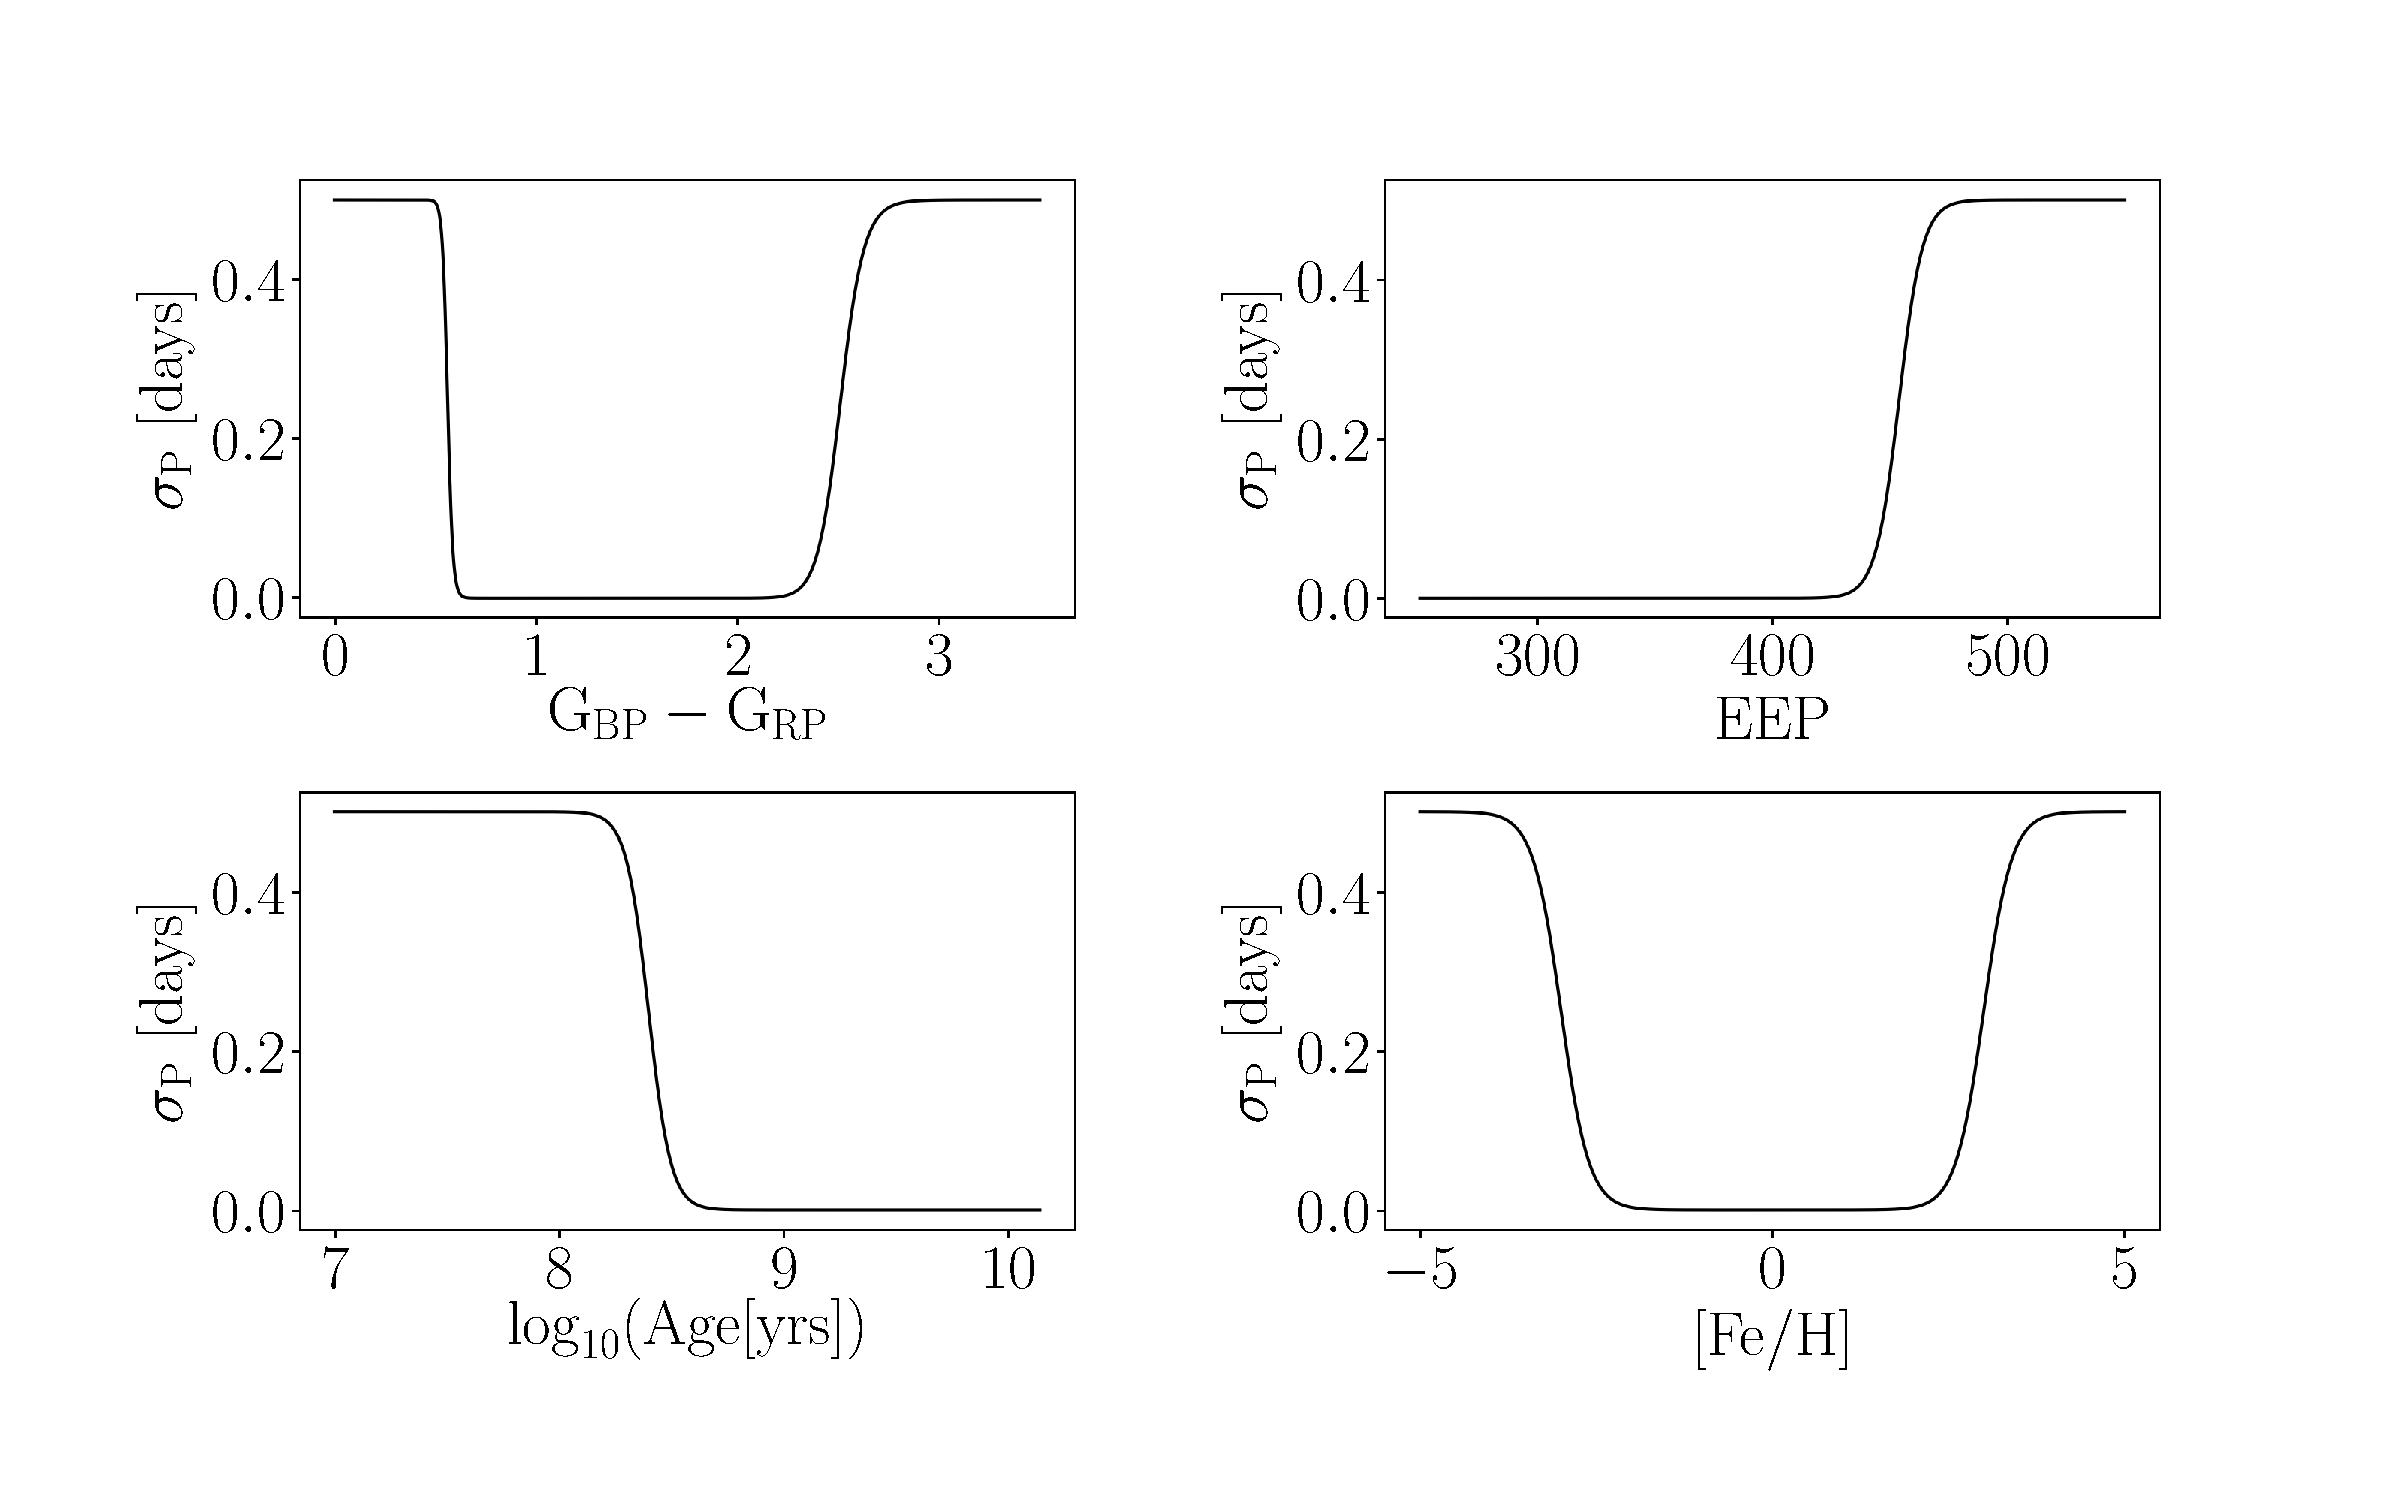
\includegraphics[width=1.\textwidth]{variance}
\label{fig:variance}
\end{figure}
Figure \ref{fig:rotation_model} shows the rotation periods of 841
stars generated from the gyrochronology model.
\begin{figure}
  \caption{
The rotation period model.
Late F, GK and early M dwarfs follow the \citet{angus2015} gyrochronology
    relation (dashed gray lines), with the exception of old, slowly
    rotating stars with large Rossby numbers whose rotation periods are fixed
    at 2$\times$ their convective overturn time.
The rotation periods of early F, late M dwarfs and subgiants were generate
    from a log-normal distribution with standard deviation shown in figure
    \ref{fig:variance}.
The top panel shows the rotation periods vs. B-V colors of simulated stars,
    colored by their age and the bottom panel shows the same stars colored
    by their equivalent evolutionary point (EEP).
    The gray lines describe \citep{angus2015} gyrochrones at ages 1, 3, 5, 7,
    9, 11, and 13 (rotation periods rise with age).
}
  \centering
    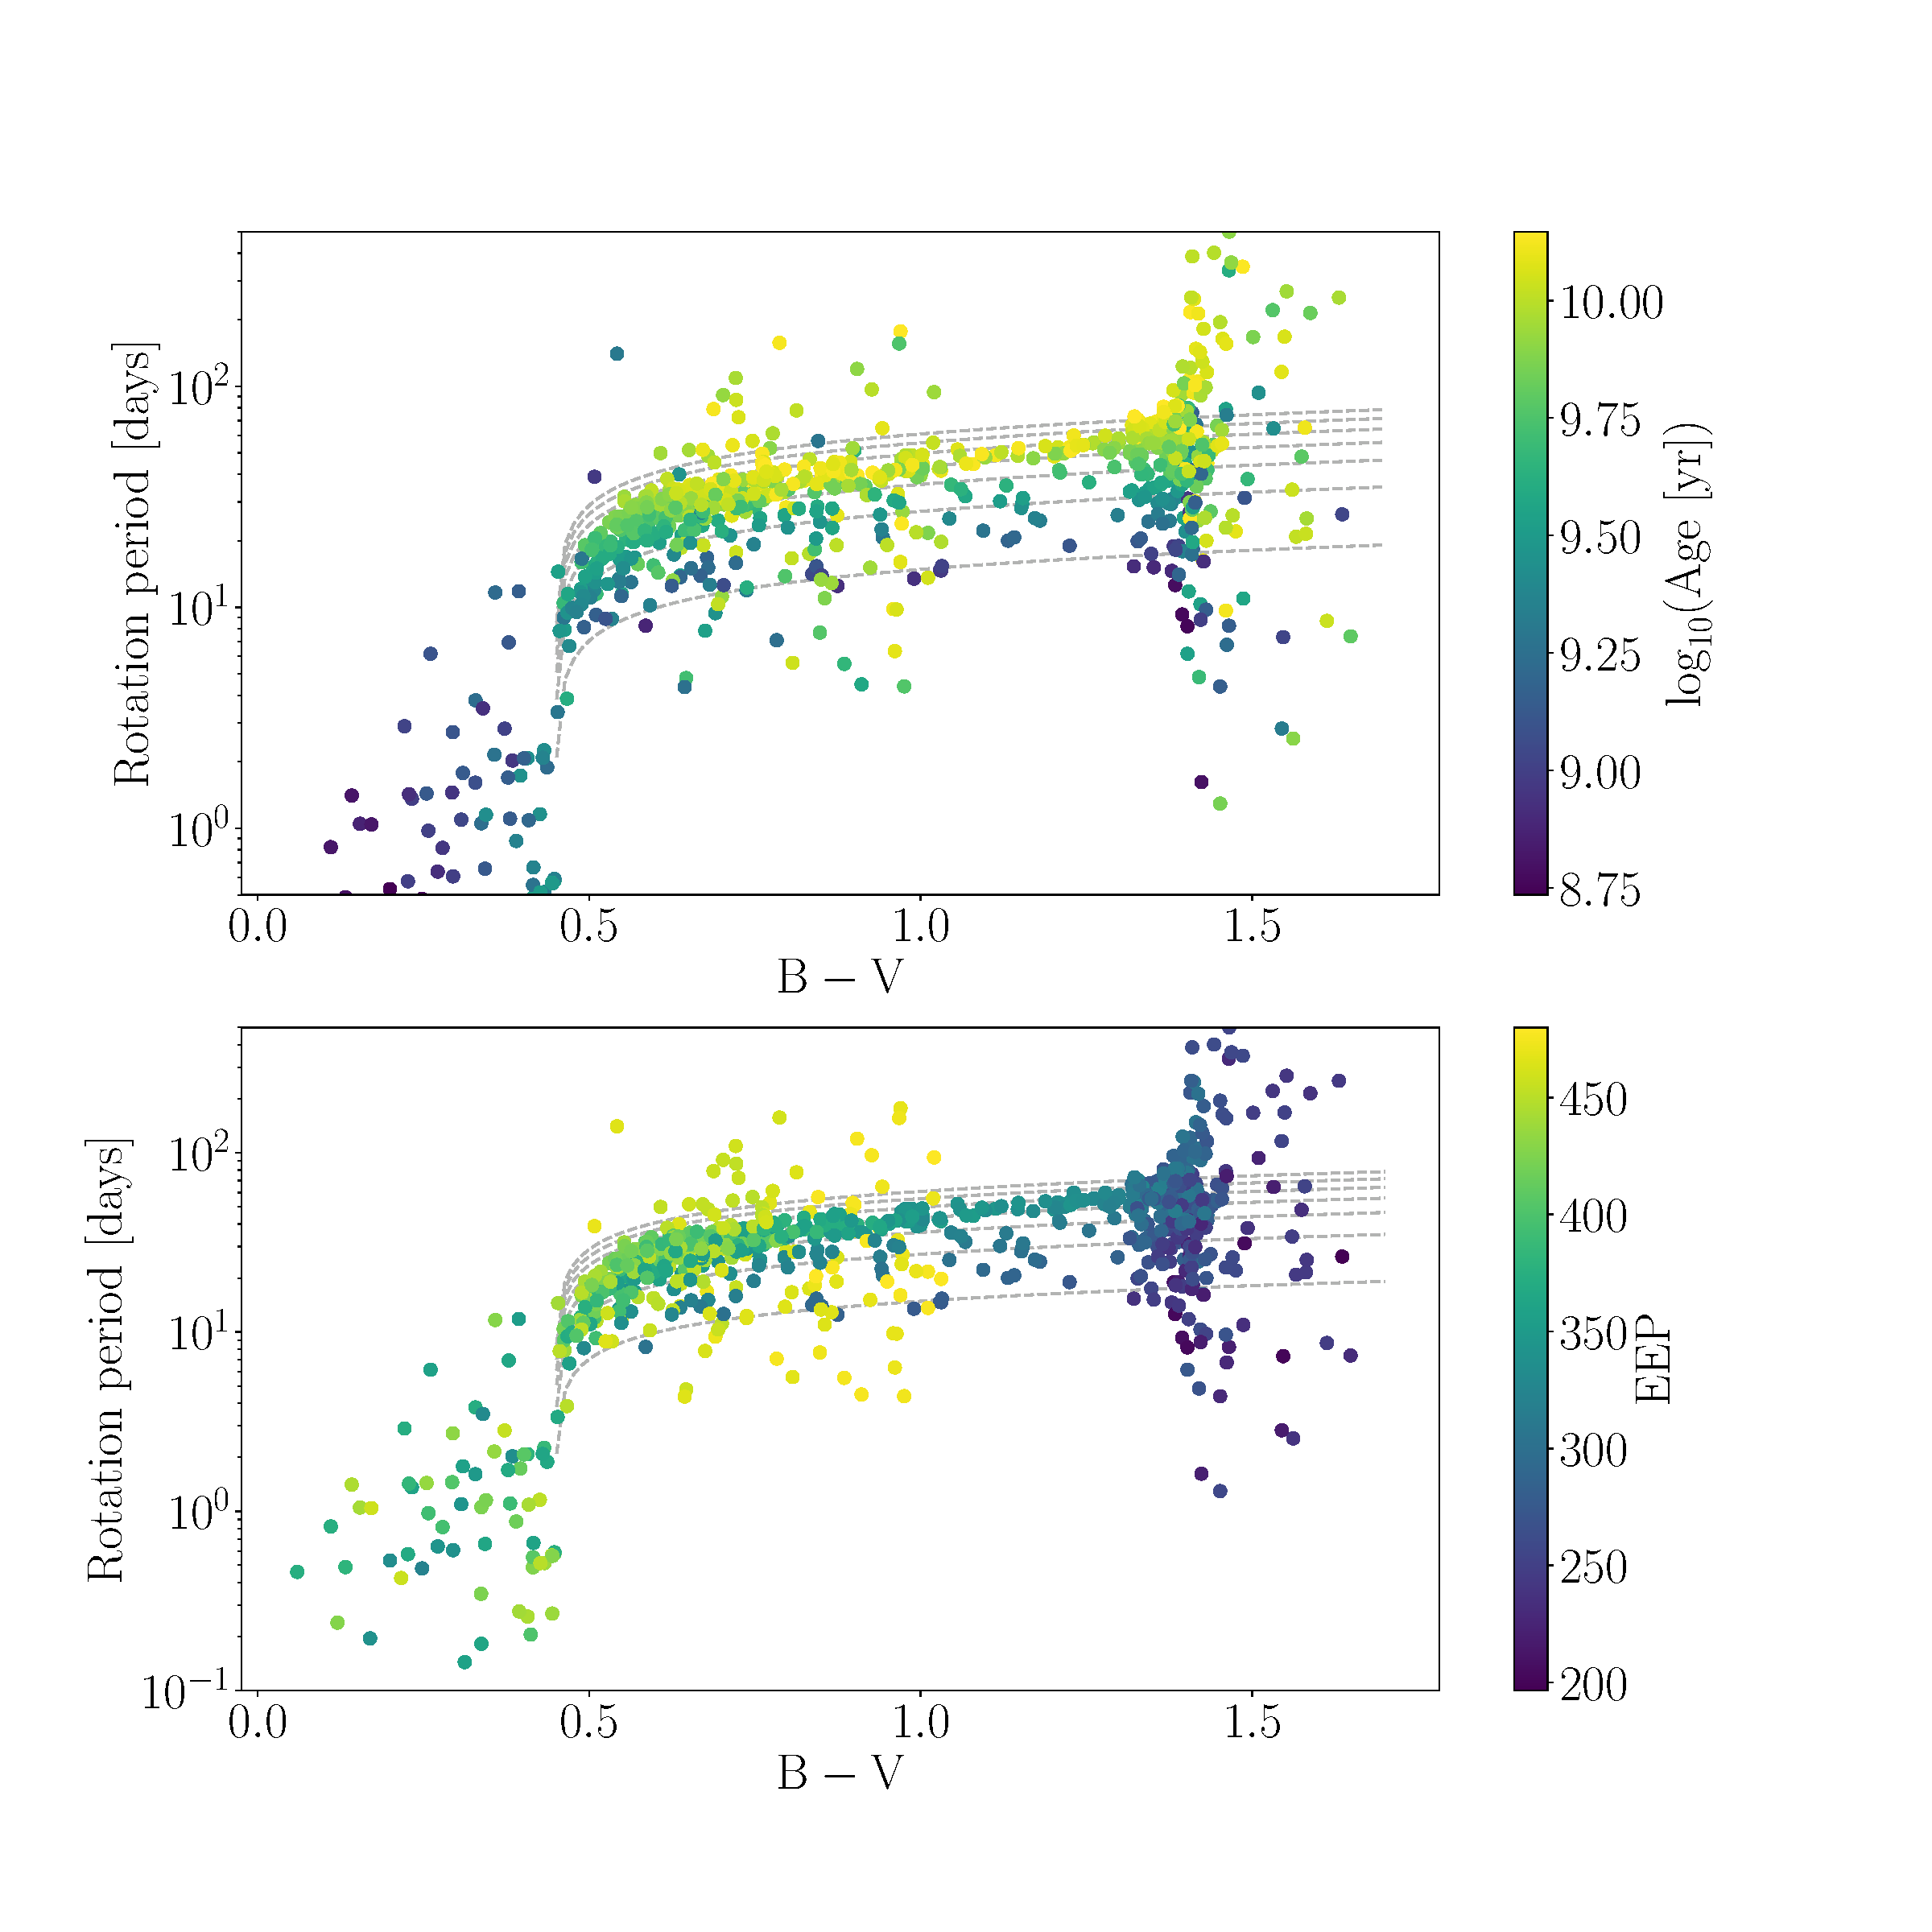
\includegraphics[width=1.\textwidth]{rotation_model}
\label{fig:rotation_model}
\end{figure}

%   - Emcee, including assessing convergence.
We sampled the joint posterior PDF over age, mass, metallicity, distance and
extinction using the affine invariant ensemble sampler, {\tt emcee}
\citep{foreman-mackey2013} with 24 walkers.
Samples were drawn from the posterior PDF until 100 {\it independent} samples
were obtained.
We actively estimated the autocorrelation length, which indicates how many
steps were taken per independent sample, after every 100 steps using the
autocorrelation tool built into {\tt emcee}.
The MCMC concluded when {\it either} 100 times the autocorrelation length was
reached and the change in autocorrelation length over 100 samples was less
than 0.01, {\it or} the maximum of 100,000 samples was obtained.
This method is trivially parallelizable, since the inference process for each
star can be performed on a separate core.
The age of a single star can be inferred in around 10 minutes on a laptop
computer.

% Although the gyrochronology model described above \citep[equation
% \ref{eqn:gyro},][]{angus2015} has been calibrated using a number of cluster
% stars, it does not provide a good fit to any individual cluster.
% No current gyrochronology model is able to capture the behavior of rotation as
% a function of color and age for individual benchmark clusters: the shape of
% this relation is different in each and current models are not flexible enough
% to capture inter-cluster differences in rotational evolution.
% For this reason, we also explored the rotational evolution of a single
% cluster, in order to produce a best-case model and demonstrate the potential
% of rotation-dating in a case where the model is perfectly accurate.
% We chose Praesepe as it is a relatively old open cluster \citep[$\sim$ 600
% Myrs][]{gossage2018}, meaning its Solar-type members have converged onto the
% rotational main sequence, and it is relatively compact on the sky so many of
% its members were observed during a single \ktwo\ campaign.
% In fact, Praesepe was repeatedly observed by \ktwo, in Campaigns 5, 16 and 18,
% however we only use rotation periods published from the analysis of Campaign 5
% in this work \citep{rebull2016}.

% % The Praesepe model
% We used a three-dimensional polynomial model to predict rotation period as a
% function of \gaia\ color and age for Praesepe and the Sun.
% This model consists of a 4th order polynomial in logarithmic Gaia color:
% $G_{Bp} - G_{Rp}$, which we write as $C_G$ for simplicity, and a 1st order
% polynomial (a straight line) in logarithmic age.
% We used \gcolor\ instead of (B-V) because, due to the $\sim$ billion stars
% observed by \gaia, it is now the most abundant and widely available
% photometric color.
% Our gyrochronology likelihood function is designed to compare observed
% rotation period to predicted rotation period.
% For this reason the gyrochronology model we used must predict rotation period
% as a function of age and color.
% However, when {\it calibrating} the gyrochronology model, we chose to make
% {\it age} the dependent variable because the uncertainties on age are much
% greater than the uncertainties on rotation period.
% Since we are using a linear model, the relation is easily invertable.
% We fit the following model to Praesepe members:
% \begin{equation}
%     \log_{10}(A) = a + b\log_{10}(C_G) + c\log_{10}^2(C_G) +
%     d\log_{10}^3(C_G) + e\log_{10}^4(C_G) + f\log_{10}(P)
% \label{eqn:gyro_age_praesepe}
% \end{equation}
% where $P$ is rotation period in days, $C_G$ is Gaia color, $A$ is stellar age
% in years and the lower case letters are free parameters which we fitted to the
% data using linear least squares.
% We adopted an age for Praesepe of 600 million years \citep{gossage2018}, a
% Solar age of 4.56 Gyr \citep{connelly2012}, and a Solar rotation period of 26
% days \citep[][Morris \etal, in prep]{balthasar1986, howe2000}.
% The Sun's color in the Gaia color bandpasses, $G_{Bp} - G_{Rp}$, is 0.82
% \citep{casagrande2018}.
% We found best-fit values: $a = 7.37 \pm 0.03, b = -1.4 \pm 0.1, c = 5.0 \pm
% 0.8, d = -34 \pm 3, e = 66 \pm 14$, and $f = 1.49 \pm 0.02$.
% Rotation periods for Prasepe were obtained from \citet{rebull2017} and their
% \gaia\ colors were obtained by crossmatching their sky-projected positions
% with the \gaia\ DR2 catalog.
% % The $f$ parameter is the inverse of the slope of the rotation period and age
% % which was originally measured to be around 0.5.
% % Our Praesepe and Sun-only fit results in a slightly steeper age dependence of
% % around 0.67, however this value is likely be
% We inverted this relation to predict rotation period as a function of color
% and age,
% \begin{equation}
%     \log_{10}(P) = \frac{\log_{10}(A) - a - b\log_{10}(C_G) - c\log_{10}^2(C_G) -
%     d\log_{10}^3(C_G) - e\log_{10}^4(C_G)}{f}.
% \label{eqn:gyro_age_praesepe}
% \end{equation}
% Both gyrochronology models of equations \ref{eqn:gyro} and
% \ref{eqn:gyro_age_praesepe} are used to predict the ages of individual
% Praesepe stars from their rotation periods and apparent magnitudes in section
% \ref{section:results}.

% % The PGM
% \begin{figure}
%   \caption{
% A probabilistic graphical model (PGM) showing the conditional
% dependencies between the parameters (white nodes) and
% observables (gray nodes) in our model.
% % ${\bf \theta}$ is a vector of {\it parameters}: mass, observed bulk
% %     metallicity, distance and V-band extinction; and ${\bf O}$ is a vector of
% %     {\it observables}: apparent magnitudes, $m_x$, effective temperature,
% %     \teff, surface gravity, \logg, observed bulk metallicity, $\hat{F}$, and
% %     parallax, $\bar{\omega}$.
% % determined by the mass, $M$, age, $A$, distance, $D$, extinction, $A_V$
% % and bulk metallicity, $F$, of a star.
% ${\bf \theta}$ is a vector of {\it parameters}: mass, observed bulk
%     metallicity, distance and V-band extinction; and ${\bf O}$ is a vector of
%     {\it observables}: apparent magnitudes, effective temperature, surface
%     gravity, observed bulk metallicity, and parallax.
%     The observables, ${\bf O}$, are determined by the parameters, $A$ and
%     ${\bf \theta}$.
%     $C_{B-V}$ is a latent parameter that is also determined by the parameters
%     $A$ and ${\bf \theta}$.
%     In our model, the rotation period observable, $P$, is determined {\it
%     only} by the age, $A$, and color ${C_{B-V}}$ parameters.
% The dependencies of observables on parameters and parameters on parameters are
%     indicated by arrows that start at a `parent' node and end at the dependent
%     observable, or `child' node.
% In our model, rotation period does not directly depend on distance,
% extinction, metallicity or mass, only age and B-V color.
% This PGM is a representation of the factorized joint PDF over parameters and
% observables of equation \ref{eqn:factorized}.
% }
%   \centering
%     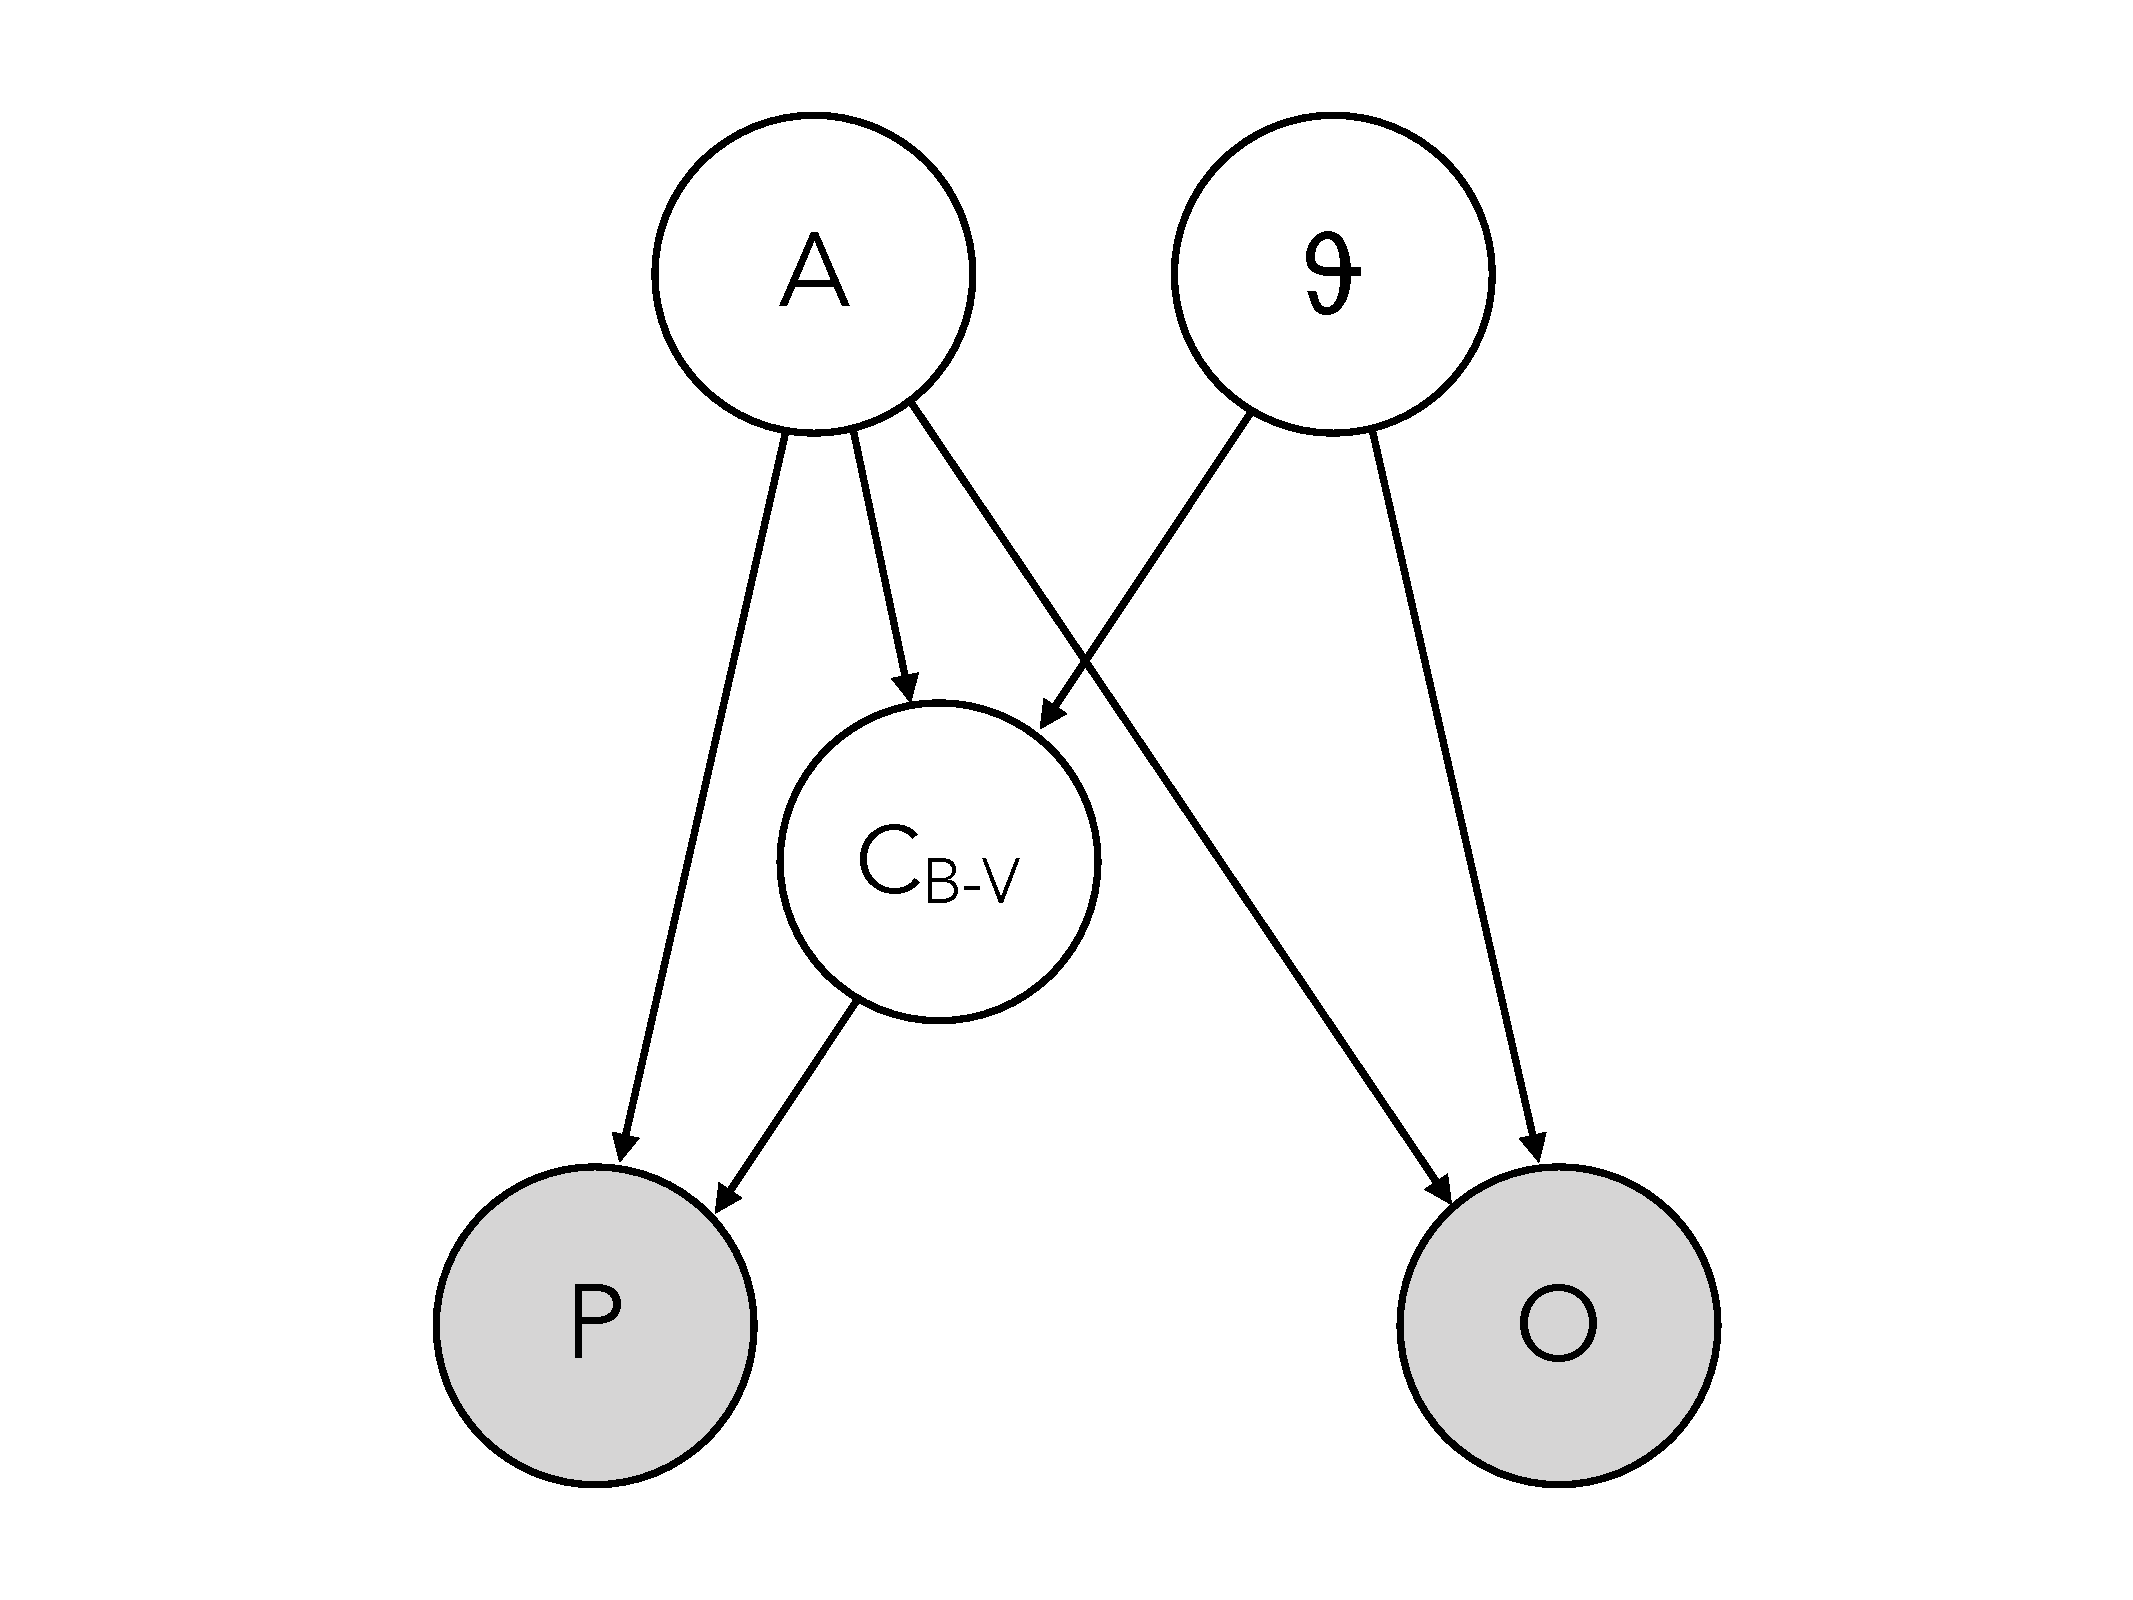
\includegraphics[width=.7\textwidth]{PGM}
% \label{fig:PGM}
% \end{figure}


% \section{Results}
% \label{section:results}
% Intro
% TEST 1: simulations
%-----------------------------------------------------------------------------
%   - The simulated data
%   - The simulation figures
%   - The results
%   - We're cheating here.
%   - Summarize and discuss the experiment.
% TEST 2: Clusters
%-----------------------------------------------------------------------------
%   - The cluster data
%   - Praesepe results: ages
%   - Praesepe results: metallicity, mass, distance
%   - Praesepe results: the Praesepe gyro relation

%   - Summary

% TEST 3: Asteroseismology
%-----------------------------------------------------------------------------
%   - The asteroseismic data
%   - The results

% TEST 4: with and without spectroscopy on simulated data.
\section{Results}
\label{section:results}

In order to demonstrate the performance of our method, we conducted two sets
of tests.
In the first we simulated a set of observables from a set fundamental
parameters for a few hundred stars using the MIST stellar evolution models and
a gyrochronology model, then compared the parameters predicted with our model
to the true parameters used to generate the data.
In the second we tested our model by attempting the measure the ages of
individual stars in the Praesepe open cluster and compared the results to the
establised age of Praesepe.
The age of Praesepe, like any open cluster, has been measured precisely
because it is an ensemble of coeval stars with the same metallicity: a single
stellar poplulation, and its age can be precisely established through
isochrone fitting and MS turn-off.
We adopted an age of 650 Myrs for Praesepe \citep{fossati2008}.

\subsection{Test 1: simulated stars}
For the first test we drew \eep s, ages, bulk metallicities, distances and
extinctions at random for 1000 stars from the following uniform distributions:
\begin{eqnarray}
& E \sim U(195, 480) \\
% & M \sim U(0.5, 1.5)~[M_\odot] \\
& A \sim U(0.5, 14)\mathrm{~[Gyr]} \\
& F \sim U(-0.2, 0.2) \\
& D \sim U(10, 1000)~\mathrm{[pc]} \\
& A_V \sim U(0, 1).
\end{eqnarray}
\teff, \logg, \fhat, \pmega\, $C_{B-V}$ and apparent magnitudes $J$, $H$ and
$K$ were generated, without noise, from these stellar parameters using the
MIST stellar evolution models.
We discarded unphysical combinations of stellar parameters, resulting in a
final sample size of 889 simulated stars.
Rotation periods were generated using the gyrochronology relation of
equation \ref{eqn:gyro}.
We took two approaches to inferring the ages of these simulated stars:
firstly using isochrone fitting {\it only}, and secondly using isochrone
fitting {\it combined with} a gyrochronology model\footnote{To infer the
ages of simulated stars, we ran our code in parallel on 100 cores. A
demonstration of this code is available at
\url{https://github.com/RuthAngus/stardate/blob/master/paper/code/simulation_results.ipynb}}.
For all stars, our initial guesses for the parameters were $E = 350$,
$A = 1$ Gyr, $F = 0$, $D = 500$ pc and $A_V = 0.1$.

%   - The results
Figure \ref{fig:iso_only} shows the results of using isochrone fitting
to estimate the posterior PDFs over the stellar ages of simulated stars.
True stellar ages are plotted on the $x$-axis and the posterior PDFs of the
inferred ages are plotted on the $y$-axis.
The rotation periods of stars were not incorporated into this model: these
posterior PDFs were obtained by isochrone fitting only, using the likelihood
function in equation \eqref{eqn:isochrones_only_likelihood}.
In most cases ages are only weakly constrained by the stellar evolution models
and in some cases there is no age constraint: the age of the star is
consistent with all ages from 0-14 Gyrs.
This is because stellar temperatures and luminosities do not change rapidly on
the main sequence: isochrones are tightly spaced there and, as a result, even
precisely measured temperatures and luminosities often do not yield precise
ages.
Figure \ref{fig:iso_and_gyro} shows the results of using isochrones {\it
combined} with a gyrochronology model.
These ages were inferred using the likelihood of equations
\eqref{eqn:full_likelihood}/\eqref{eqn:both_likelihood}.
Again, figure \ref{fig:iso_and_gyro} shows true stellar ages on the $x$-axis
and the posterior PDFs of the inferred ages on the $y$-axis.
Here, unlike the isochrone only case, the recovered ages are precise because
there is more age information in stellar rotation periods than in effective
temperatures and absolute magnitudes.
Gyrochronology isochrones (or gyrochrones) are more widely separated relative
to the observational uncertainties than the MIST isochrones.
Put another way, the rotation periods of two stars of different ages and the
same mass will have rotation periods that differ significantly -- almost
certainly more than the observational uncertainty on rotation period.
On the other hand, such stars are likely to have extremely similar
luminosities and temperatures and the differences between these properties are
likely to be smaller than the observational uncertainties.

Figures \ref{fig:iso_precision} and \ref{fig:gyro_precision} show the
simulated stars on a color magnitude diagram, colored by the relative
precision of their predicted ages.
Figure \ref{fig:iso_precision} shows age precision as a function of CMD
position using isochrone fitting only, and figure \ref{fig:gyro_precision}
shows age precision using isochrone fitting and gyrochronology combined.
These figures are semi-empirical versions of figures \ref{iso_fisher} and
\ref{gyro_fisher}, which were created using information theory, and show the
theoretical minimum precision of isochrone fitting and gyrochronology.
\racomment{Still to do: add these figures!}

% We're cheating here.
% Figure \ref{gyro_only} demonstrates the results of inferring ages using
% rotation periods only, and this illustrates why the combination of isochronal
% and gyrochronal ages is so precise: almost all this precision comes from
% rotation periods.
This simulation experiment is unrealistic for two main reasons: firstly, we
simulated data from the same gyrochronology model we used to infer ages and so
the results will be perfectly accurate by design.
Secondly, we simulated data without any intrinsic scatter built into the
gyrochronology model; it is a deterministic model.
This means that a rotation period and color predicts a corresponding
single-valued age, rather than a probability distribution over ages.
This is unrealistic given observations of open clusters whose members clearly
show excess scatter in their rotation periods, particularly for less massive
stars (see figure \ref{fig:praesepe}).
These results look precise and accurate, but this is misleading.
Inaccuracies would arise if the gyrochronology model was incorrect or poorly
calibrated in some areas of parameter space and imprecision would arise if
intrinsic scatter were built into the gyrochronology model and/or the
observations.
The result of using a deterministic model, such as the one used in this
experiment, is that the uncertainties on stellar ages will be unrealistically
small.
We leave the recalibration of gyrochronology models for a future exercise
since, in this work, we are mostly interested in testing the results of simply
combining gyrochronology and isochrone fitting.
The above experiment shows that building gyrochronology into stellar evolution
models results in much more precise age predictions, as predicted by
information theory.
We have not yet made any statement about accuracy however; the above
experiment produces accurate ages by construction.
In order to test the accuracy of this method, we tested it on real data: the
Praesepe open cluster.

% TEST 2: Clusters
%-----------------------------------------------------------------------------
%   - The cluster data
\subsection{Test 2: the Praesepe Cluster}
In order to test our model on real stars with known ages, we selected a sample
of cluster stars with precisely measured ages from ensemble isochrone fitting
and main sequence turn off.
The ages of open clusters can be measured much more precisely than field
stars.
Stars in the same cluster formed (we assume) from the same molecular cloud at
the same time and therefore have the same metallicity and age (to within a few
million years).
Stars with the same metallicity and age fall on the same isochrone,
allowing perfect isochrone selection and providing a $N^{-1/2}$ decrease in
uncertainty where N is the number of cluster stars.
Single stellar populations also allow main sequence turn off to be identified
and, as demonstrated in figure \ref{fig:iso_fisher}, the turn off supplies a
large amount of age information.
We compiled rotation periods, \Gaia\ photometry and \gaia\ parallaxes for
members of Praesepe, a $\sim$650 Myr cluster \citep{fossati2008}.
We chose Praesepe because it is relatively tightly clustered on the sky and
many of its members were targeted in a single \ktwo\ campaign, from which it
was possible to measure rotation periods via frequency analysis of member's
light curves \citep{douglas2017}.
We crossmatched Praesepe members with measured rotation periods
\citep{douglas2017} with the Gaia DR2 catalog \citep{brown2018}, using a 1''
search radius.
The result was a sample of 757 stars with rotation periods, parallaxes and
\gaia\ $G$, $G_{BP}$ and $G_{RP}$-band photometry.
Figure \ref{fig:praesepe} shows the rotation periods of Praesepe members as
a function of their \gaia\ \gcolor\ colors.
The GK and early M dwarfs (\gcolor\ $<$ 2.4) which fall on a `rotational main
sequence' are shown as blue points and the late M dwarfs (\gcolor\ $>$ 2.4)
whose rotation periods are not well determined by their age and color are
shown as orange open circles.
We excluded the late M dwarfs (orange circles with \gcolor\ $>$ 2.4) from this
analysis since they do not follow a simple gyrochronology relation however, we
included more massive outliers (orange circles with \gcolor\ $<$ 2.4) in order
to provide a complete picture of the precision and accuracy of gyrochronology
applied to Praesepe.
Figure \ref{fig:praesepe} shows two sets of gyrochronology models: one
calibrated using several open clusters, asteroseismic stars and the Sun
\citep{angus2015}, which was used to infer the ages of Praesepe but clearly
does not provide a perfect fit to this cluster (solid gray line), and one fit
to Praesepe and the Sun only, as described in section
\ref{section:motivation}, that was used to calculate the Fisher information
(dashed black line).
We did not account for extinction in our analysis since Praesepe is relatively
nearby (around 180 parsecs) so reddening from dust is minimal.

% The age of each Praesepe member was inferred using both of these
% gyrochronology models: the legacy model of equation \ref{eq:gyro} and the
% Praesepe model of equation \ref{eq:new_gyro}.
% This exercise is not designed to test one gyrochronology model against
% another: the model fit to the Praesepe data will provide a better age
% prediction by design, as the legacy model was fit to number of clusters at
% once.
% The point of this exercise is to show how precise gyrochronology could be if
% a {\it perfect} model was used.
% The age of each Praesepe member was inferred using our combined stellar
% evolution and gyrochronology model.
% We did not force the cluster members to have the same age since the aim of
% this experiment was to reveal the precision and accuracy of our method by
% quantifying the level of scatter in our predicted ages and identifying regions
% of parameter space where the ages deviate from the established age for
% Praesepe.

%   - Praesepe results: ages
The resulting probability density functions over age predicted for individual
members of Praesepe, where each member was treated as an isolated field star,
are shown in figure \ref{fig:ages}.
The orange distributions show posterior PDFs over age for each member of
Praesepe, where ages were inferred using isochrone fitting {\it only},
with \gaia\ colors (\gcolor), \gaia\ apparent magnitude ($G$), and \gaia\
parallaxes as the observable properties.
The blue distributions are posterior PDFs over stellar age for each member of
Praesepe, where ages were inferred using isochrone fitting {\it and}
a gyrochronology model (equation \ref{eqn:gyro}).
The blue posteriors are much more strongly peaked around the literature age of
the cluster (650 Myrs, indicated by a vertical black line) and this
demonstrates that rotation periods carry far more age information than
photometric colors, even when precise parallaxes are available.
\racomment{Still to do: calculate summary statistics describing the precision
improvement.}

% % Cutting outliers and limiting color range.
% In order to fit a period-color relation to these data we restricted the sample
% of cluster stars to the color range, 0.56 $<$ \gcolor\ $<$ 3 in order to
% remove early F and late M dwarfs whose rotation periods do not fall on the
% `gyrochronology main sequence'.
% Although it {\it may} be possible to crudely predict the ages of these stars
% (at least the M dwarfs) from their rotation periods, the age-rotation-color
% relation for these stars is very different to the FGK star relations and is
% not the focus of this paper.
% In addition, we removed rapidly rotating stars from the sample since, although
% modeling outliers is important and consequential for gyrochronology in
% general, the goal of this paper is not to produce a perfect gyrochronology
% that reproduces stochasticity in the data, just a simple function that fits
% the rotational main sequence of Praesepe.
% In future we plan to update the gyrochronology models to include M dwarfs,
% and the outlying rapid rotators using a mixture of Gaussians.
% Similarly, we used only Praesepe in this study because the period-color
% relations of each open cluster with rotation periods has a different shape.
% This is likely due to differences in metalicities, incomplete or noisy
% membership lists and differences in rotation period measurement algorithms.
% A global gyrochronology calibration, using all cluster data is planned for the
% future but, again, is beyond the scope of the project presented here.
% The rotation periods of the Praesepe members in the restricted color range and
% with outliers removed are plotted against their \Gaia\ colors in figure
% \ref{fig:Praesepe}.
% We used linear least squares to fit a linear model to Praesepe and the Sun.
% A 4th order polynomial in $\log(G_{BP} - G_{RP})$ and a straight line in
% $\log(\mathrm{Age~[yrs]})$ was fit to reproduce
% $\log(\mathrm{rotation~period~[days]})$.
% \begin{equation}
%     \log(P) = a + b\log(C_G) + c\log^2(C_G) + d\log^3(C_G) + e\log^4(C_G) +
%     f\log(A),
% \end{equation}
% \label{eq:new_gyro}
% were $P$ is period, $C_G$ is \Gaia \gcolor\ color, and A is age.

% %   - Praesepe results: metallicity, mass, distance
% Stellar rotation periods are age-informative and so including them in our
% analysis leads to the more precise measurement of ages.
% However, rotation periods do not carry very much information about the
% metallicity of a star, nor their distance.
% They are also not particularly informative about the mass of a star because,
% even though rotation period depends on both mass and age, stellar mass is
% strongly informed by color and temperature information, so is chiefly
% determined by the stellar evolution/isochrone models.
% However, age, mass and metallicity are correlated: a star can be more blue
% because it is more massive, older or more metal poor and for this reason, if a
% star's age is more tightly constrained, constraints on its mass and
% metallicity will also improve.
% Figures \ref{fig:metallicity} and \ref{fig:mass} show the differences in
% posterior PDFs over metallicity and mass respectively, calculated for Praesepe
% stars where rotation period information is both used (blue posteriors) and not
% used (orange posteriors).
% The black line in figure \ref{fig:metallicity} shows the established
% metallicity of Praesepe \racomment{citation}.
% There is little difference between blue and orange because rotation periods do
% not strongly depend on metallicity or mass (independantly of age).
% However, the precision of mass and metallicity measurements are slightly
% improved due to the fact that age, mass and metallicity are correlated.
% Figure \ref{fig:distances} shows the posterior PDFs over distance to the
% Praesepe cluster.
% In this example of fitting our model to Prasepe data, Since we used \gaia\
% parallaxes, which are extremely informative about distances, more precisely
% constrained ages make a minimal improvement to distances.

%   - Praesepe results: the Praesepe gyro relation
% The results in figure \ref{fig:praesepe_old_model_ages} were produced using a
% gyrochronology relation (equation \ref{eqn:old_gyro}) that was calibrated
% using the Hyades, Coma Berenices and Pleiades clusters, plus the Sun and old
% asteroseismic stars \citep{angus2015}.
% Figure \ref{fig:praesepe_new_model_ages} however, shows the results of
% inferring the ages of Praesepe members with the dedicated Praesepe
% gyrochronology relation of equation \ref{eqn:gyro_age_praesepe}.
% We include these results because we would like to provide an idea of the kind
% of age measurement accuracy that is achievable in the best case: where the
% gyrochronology model perfectly reproduces the data.

%   - Summary
In summary, fitting our new age model to simulated stars and members of the
Praesepe cluster (an open cluster with a precisely measured age from ensemble
isochrone fitting and MS turn-off) demonstrates that using isochrone fitting
{\it alone} to calculate the ages of cool MS field stars results in
extremely imprecise ages, however when gyrochonology is incorporated, the
precision of age measurements increase significantly.

% The simulation figures
% iso only
\begin{figure}
  \caption{
The results of a test in which we simulated observable properties of stars
    with the same model we used to infer their properties.
In this experiment we used {\it only} isochrone fitting to infer ages;
we did not use rotation periods/gyrochronology.
    For results where we used {\it both} stellar evolution models {\it and}
    gyrochronology, see figure \ref{fig:iso_and_gyro}.
The true age, used to produce associated observables is shown on the x-axis,
    and the inferred ages are shown on the y-axis.
This figure shows the posterior PDFs over stellar age for each of the
    simulated stars as a `violin plot', where samples from the posterior are
    plotted vertically as a smooth, symmetric function.
The widths of these functions indicates the probability density over age:
    wider regions indicated greater probability mass.
The median values of the posterior PDFs are plotted as solid horizontal lines.
This figure demonstrates that when only stellar evolution models are used to
    infer ages for field MS stars, the resulting predicted ages are extremely
    imprecise.
}
  \centering
    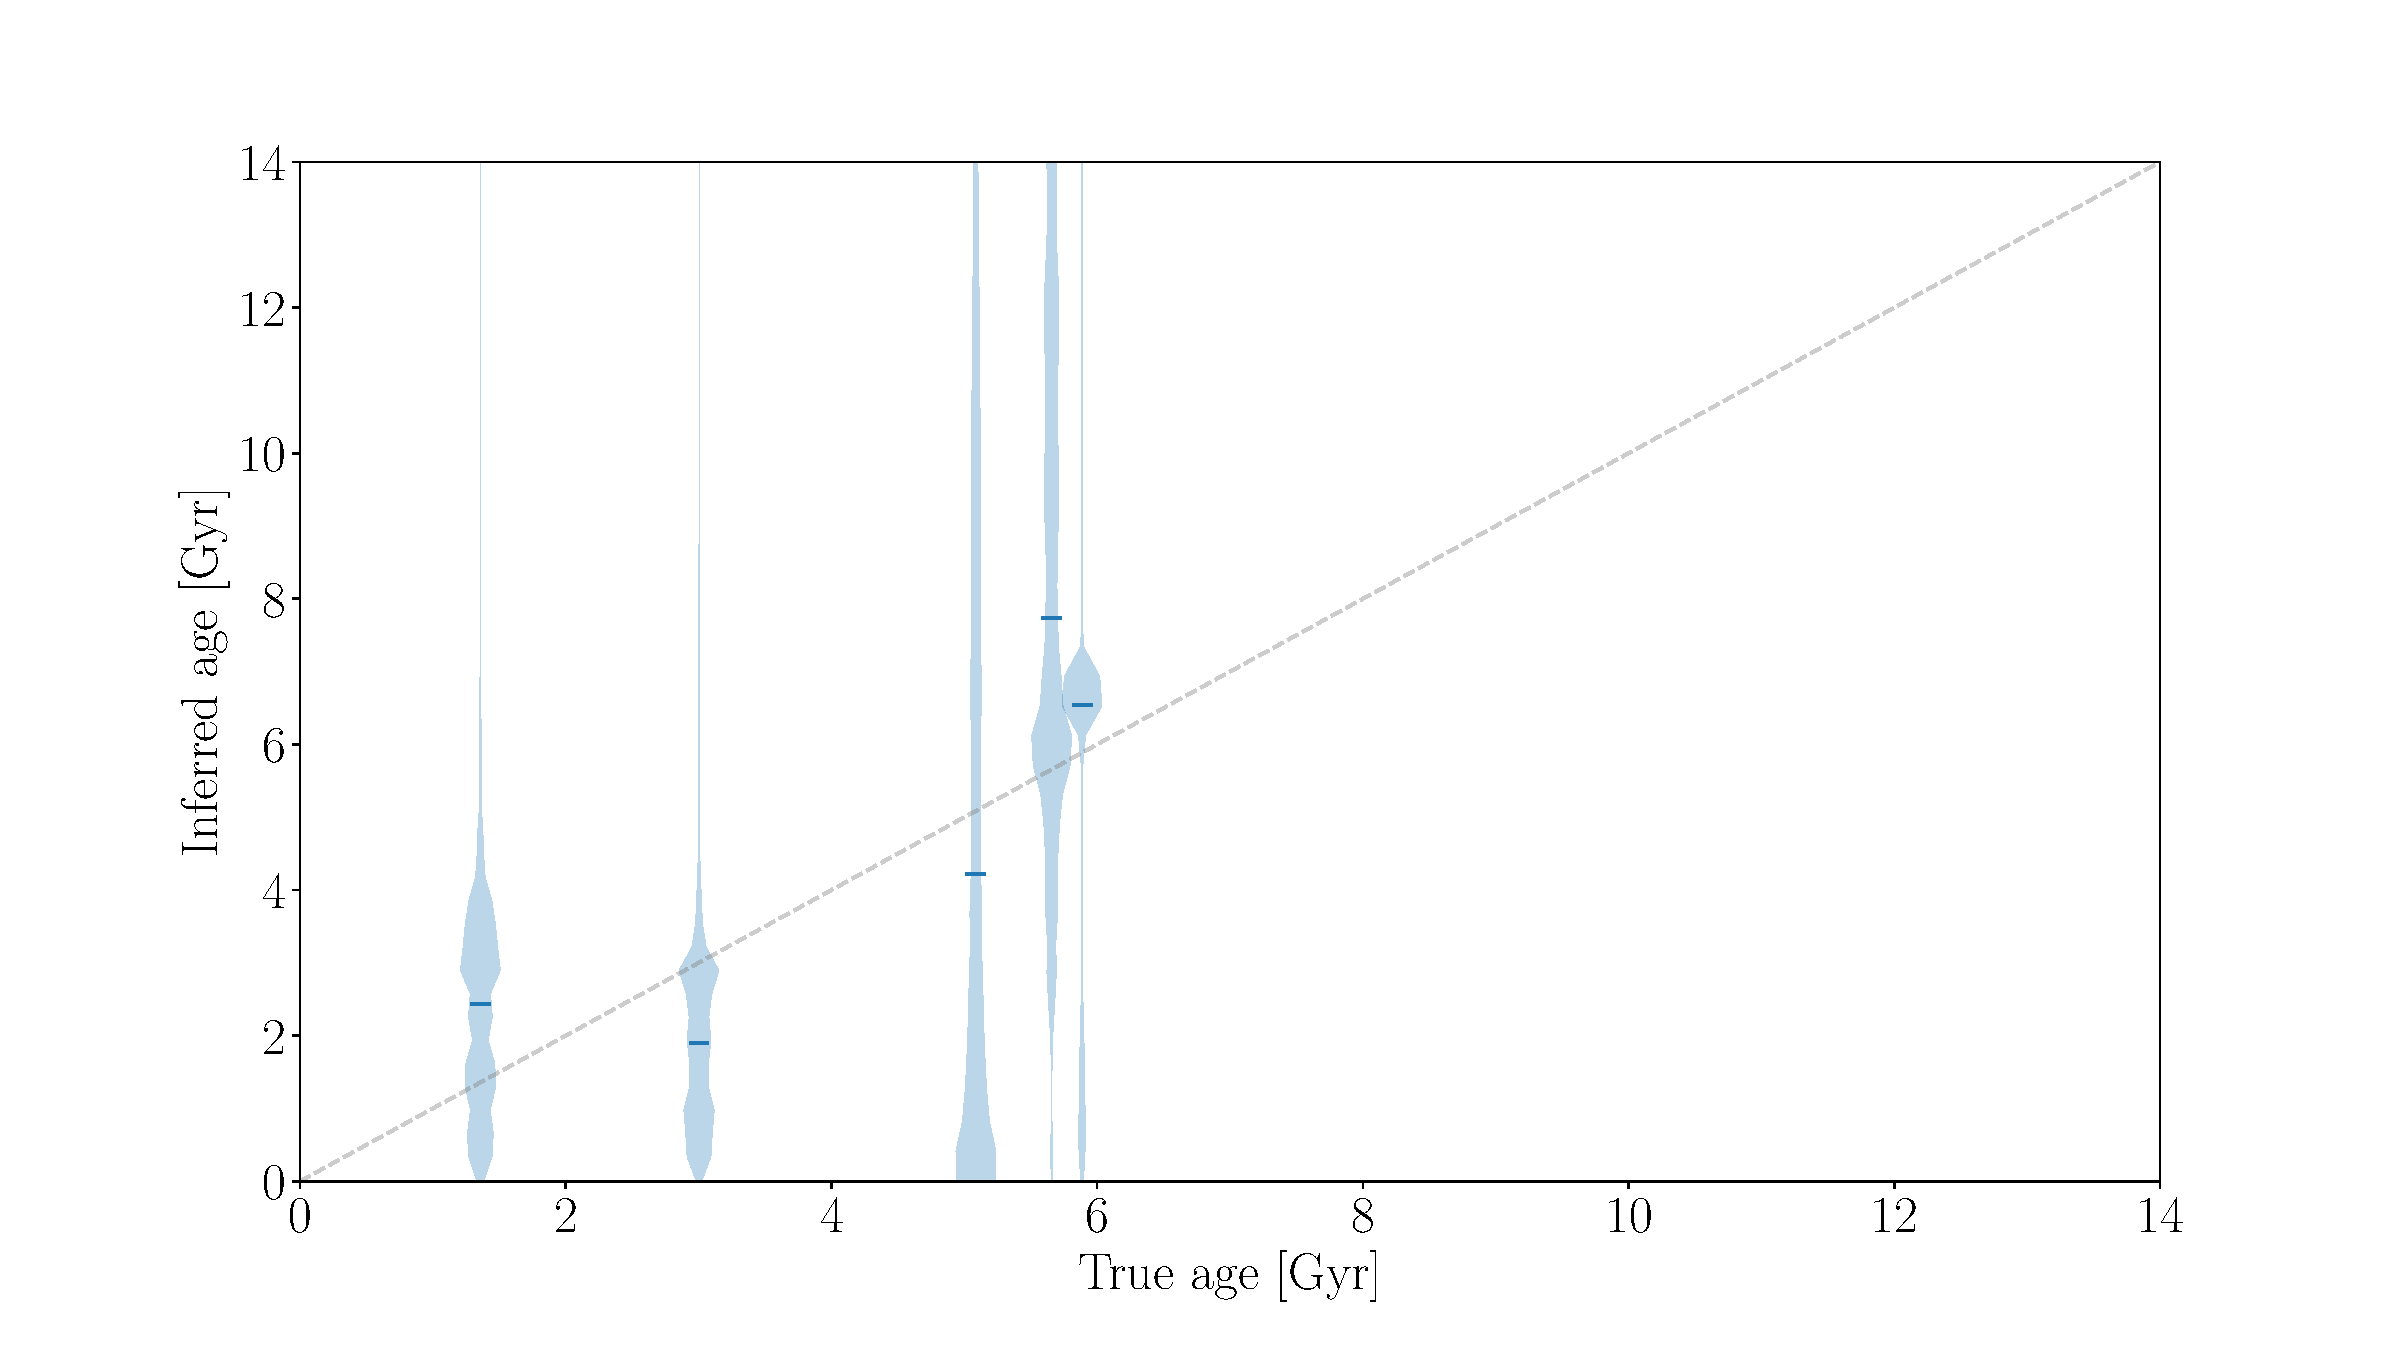
\includegraphics[width=1\textwidth]{../plots/iso_only_violin.pdf}
\label{fig:iso_only}
\end{figure}

\begin{figure}
  \caption{
The results of a test in which we simulated observable properties of stars
    with the same model we used to infer their properties.
    In this experiment we used both isochrone fitting {\it and}
    gyrochronology to infer ages.
For results where we used stellar evolution models {\it only}, see the
    previous figure (figure \ref{fig:iso_only}).
The true age, used to produce associated observables is shown on the x-axis,
    and the inferred ages are shown on the y-axis.
This figure shows the posterior PDFs over stellar age for each of the
    simulated stars as a `violin plot', where samples from the posterior are
    plotted vertically as a smooth, symmetric function.
The widths of these functions indicates the age probability density: wider
    regions represent greater probability mass.
The median values of the posterior PDFs are plotted as solid horizontal lines.
    This figure demonstrates that when rotation periods (gyrochronology) {\it
    and} stellar evolution models are used to infer the ages of field MS
    stars, the resulting predicted ages are much more precise
    than isochrone fitting can provide alone.
    \racomment{I am rerunning code to fix the outliers in this figure -- I
    think it's an initialization issue. I am also planning to combine this
    figure with the figure above.}
}
  \centering
    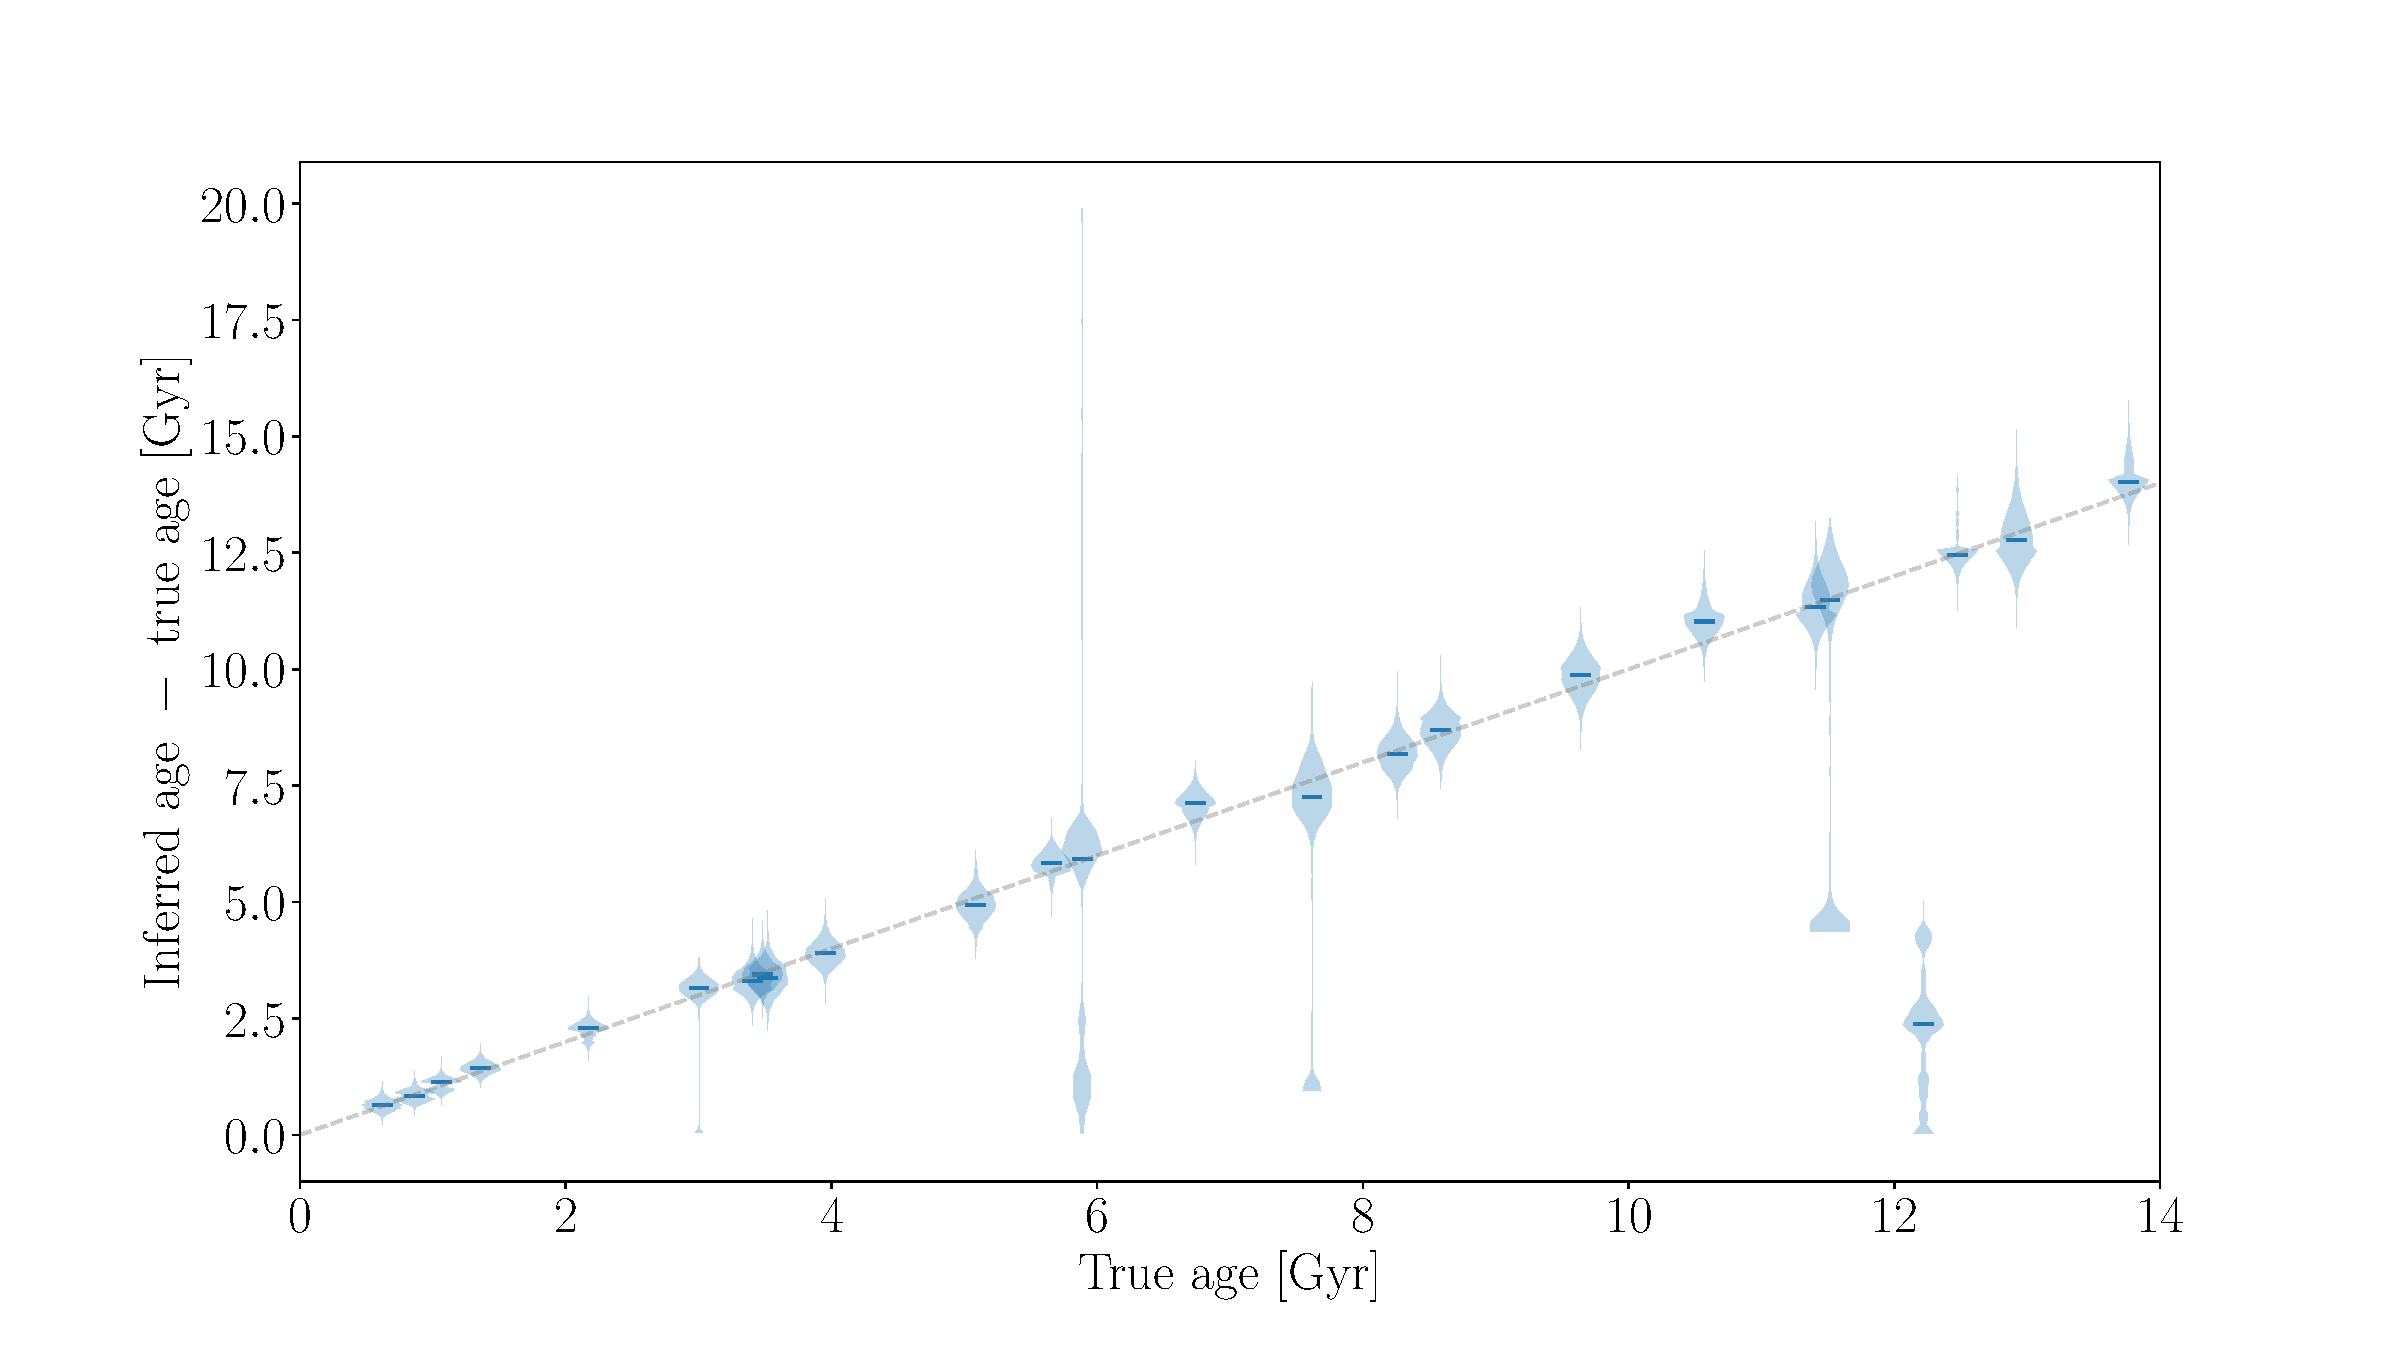
\includegraphics[width=1\textwidth]{../plots/iso_and_gyro_violin.pdf}
\label{fig:iso_and_gyro}
\end{figure}

% % The Cluster figure
% \begin{figure}
%   \caption{
% % The rotation periods of stars in open clusters, and the Sun, plotted against
% %     their \Gaia\ colors (\gcolor) in logarithmic space.
% % The result of this fit is plotted on top of the data at the ages of
% %     the cluster stars and the Sun.
%     The rotation periods of Praesepe members and the Sun, plotted against
%     their \Gaia\ colors (\gcolor) in logarithmic space.
%     We fit a linear model to these data in order to predict
%     rotation periods from \gaia\ colors and age.
%     This model consisted of a fourth-order polynomial in $\log_{10}$ color,
%     and a 1st order polynomial (a straight line) in $\log_{10}$ age.
% The result of this fit is plotted on top of the data at the ages of
%     Praesepe and the Sun.
% }
%   \centering
%     \includegraphics[width=1\textwidth]{clusters.pdf}
% \label{fig:clusters}
% \end{figure}

\begin{figure}
  \caption{
    The rotation periods of Praesepe members \citep{douglas2016}, plotted
    against their \Gaia\ colors (\gcolor) in logarithmic space.
    GK and early M dwarfs (\gcolor\ $<$ 2.4), shown as blue points fall on a
    `rotational main sequence' whereas the rotation periods of late M dwarfs
    (2.4 $<$ \gcolor), shown as orange open circles
    are noisy and not strongly predicted by their age and color.
    We excluded late M dwarfs from our age analysis of Praesepe stars.
    We excluded outliers at earlier spectral types, also shown as open orange
    circles at colors less than 2.4, to perform the polynomial fit to Praesepe
    described in section \ref{section:motivation} (resulting in the black
    dashed line) but included these outliers when inferring the ages of
    Praesepe stars in section \ref{section:results}.
    The early-type outliers were identified via sigma-clipping at
    4.5$\sigma$.
    The black-dashed model was used to calculate the Fisher information shown
    in figures \ref{fig:iso_fisher} and \ref{fig:gyro_fisher}.
    The solid gray lines show gyrochrones that were calibrated using the
    Hyades, Coma Berenices and Pleiades clusters, as well as the Sun and
    \kepler\ asteroseismic stars \citep{angus2015}, and used to predict the
    ages of Praesepe stars, shown in figure \ref{fig:cluster_ages}.
    This model does not provide a perfect fit to Praesepe (Praesepe was not
    used to calibrate it),
    particularly for the hottest and coolest stars,
    however this is the current gyrochronology model implemented in our joint
    isochrone fitting and gyrochronology model.
    This figure was generated in a {\it Jupyter} notebook available at this
    url:
https://github.com/RuthAngus/stardate/blob/master/paper/code/Praesepe.ipynb
}
  \centering
    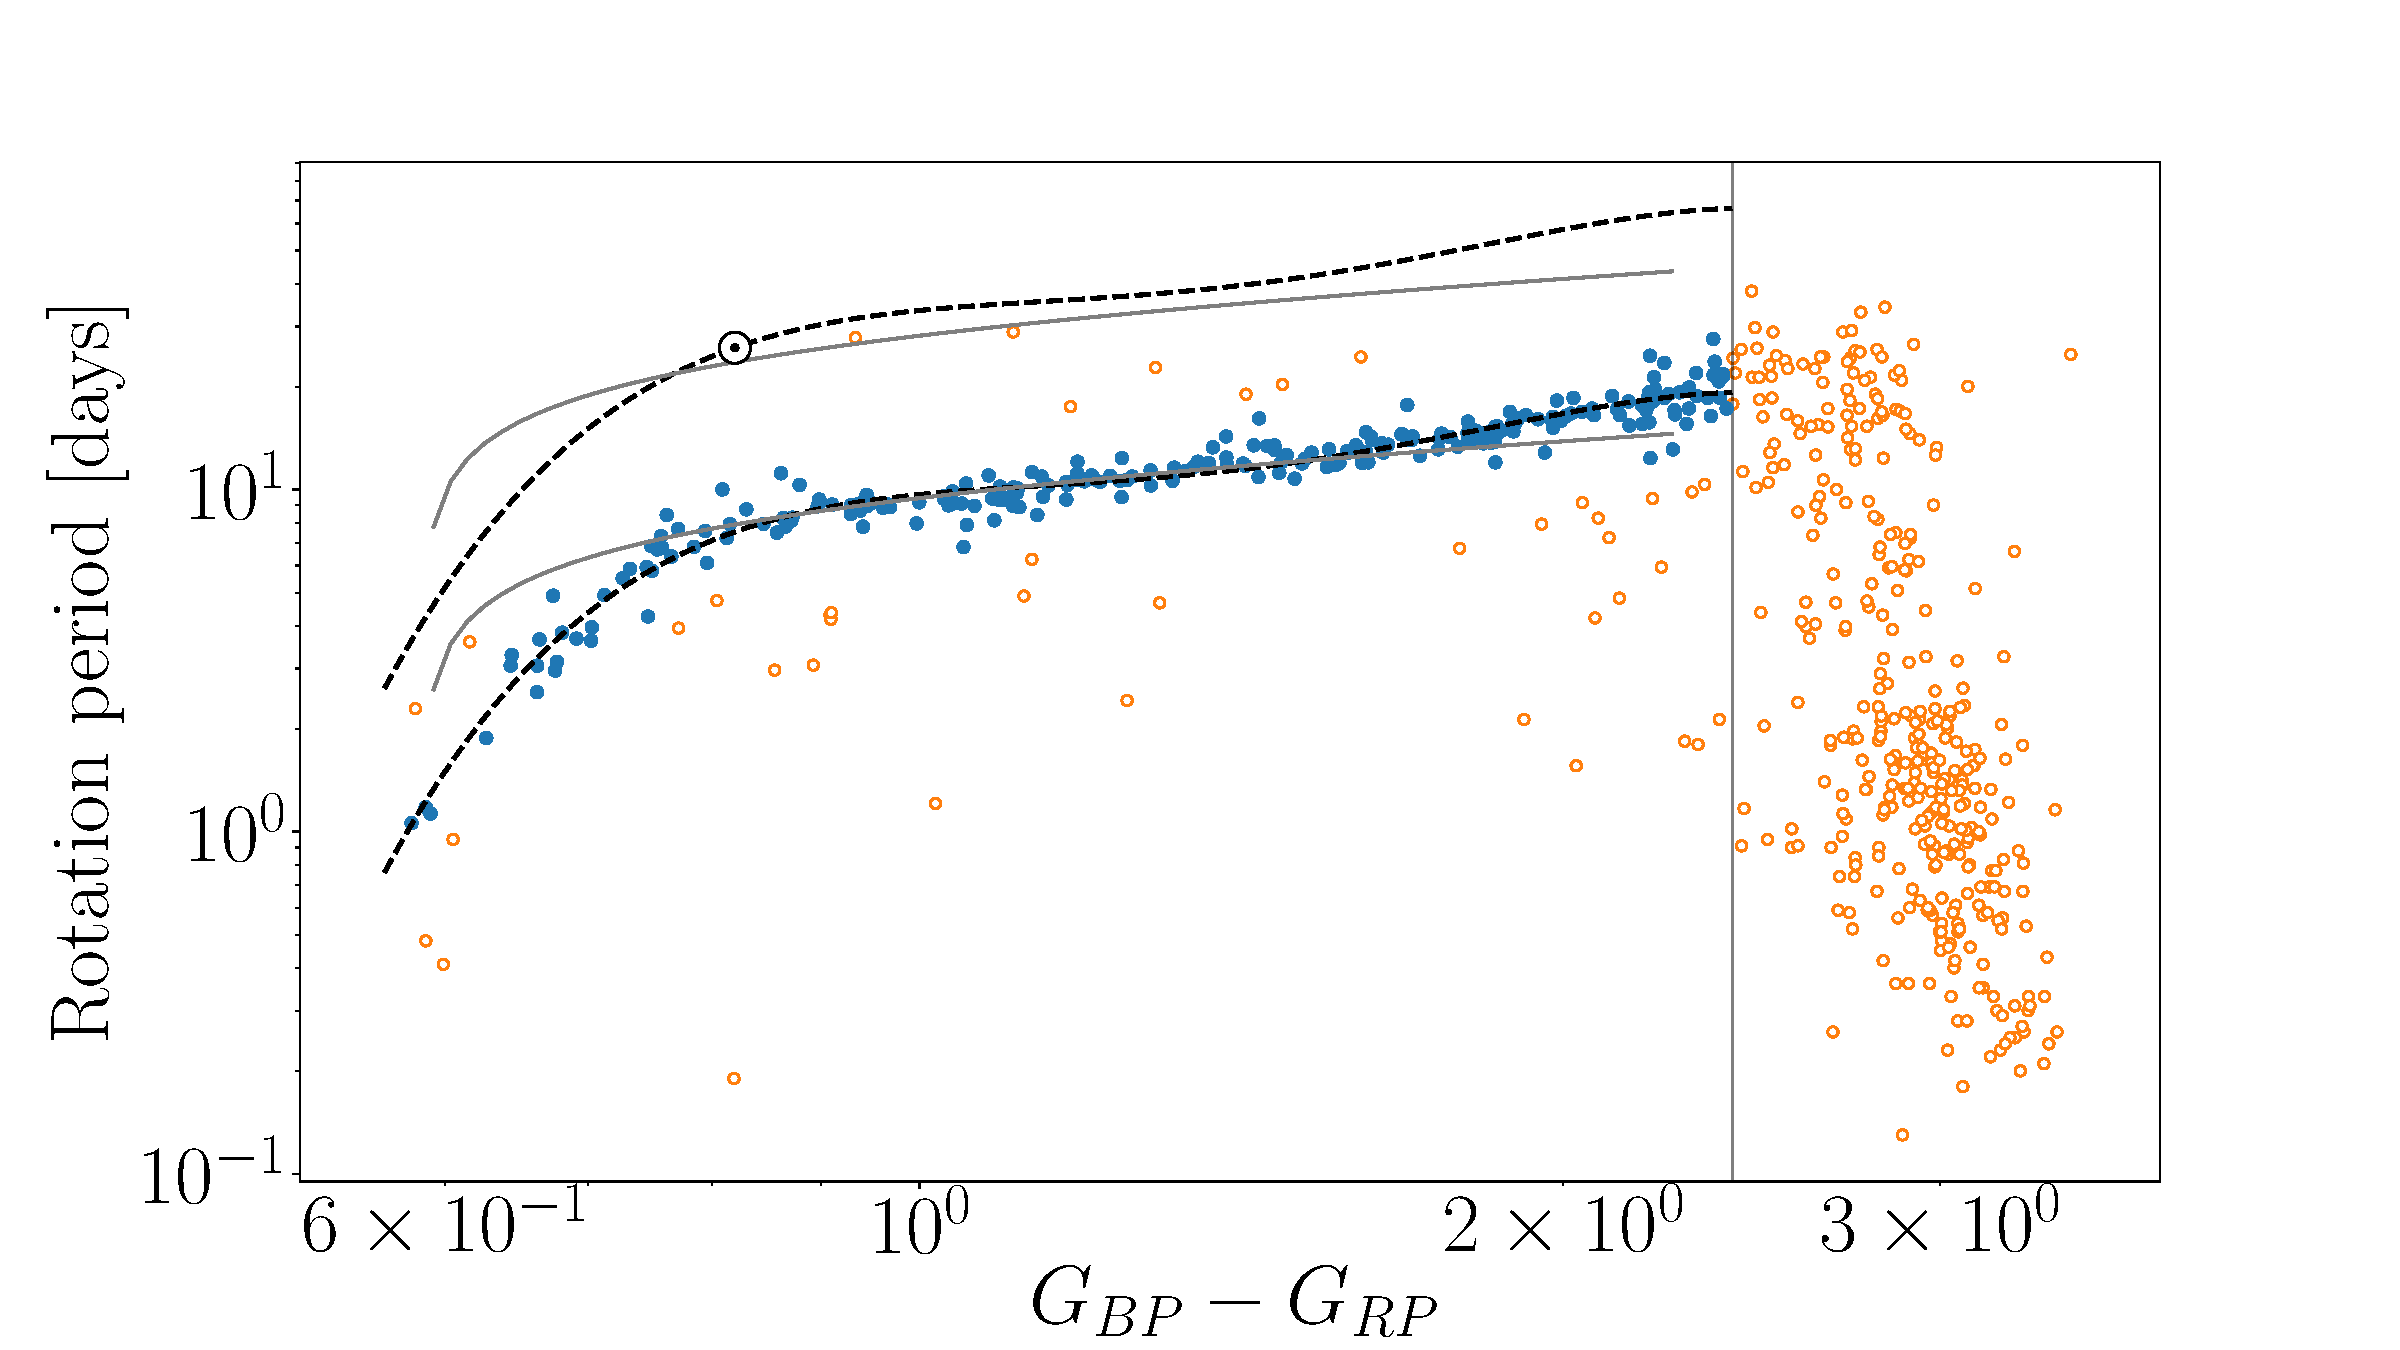
\includegraphics[width=1\textwidth]{with_angus_gyrochrones.pdf}
\label{fig:praesepe}
\end{figure}

\begin{figure}
  \caption{
    The unnormalized posterior PDFs over the ages of Praesepe stars inferred
    using an isochrone fitting method (orange) and a joint isochrone fitting
    and gyrochronology model (blue).
    MIST isochrones were used for isochrone fitting and the gyrochronology
    model is shown as solid grey lines in
    figure \ref{fig:praesepe} \citep{angus2015}.
    The black line shows the established age of Praesepe (650 Myrs).
    The blue posterior PDFs are more strongly peaked around the established
    age for Praesepe than the orange, indicating that gyrochronology is much
    more informative for these MS stars than isochrone fitting.
    \racomment{Still need to quantify the improvement}
}
  \centering
    \includegraphics[width=1\textwidth]{cluster_ages.pdf}
\label{fig:cluster_ages}
\end{figure}


% \begin{figure}
%   \caption{
%     The posterior PDFs over metallicity of Praesepe stars inferred using an
%     isochrone fitting method (orange) and a joint isochrone fitting and
%     gyrochronology model (blue).
%     The black line shows the established metallicity of Praesepe (citation).
%     The blue posterior PDFs are
% }
%   \centering
%     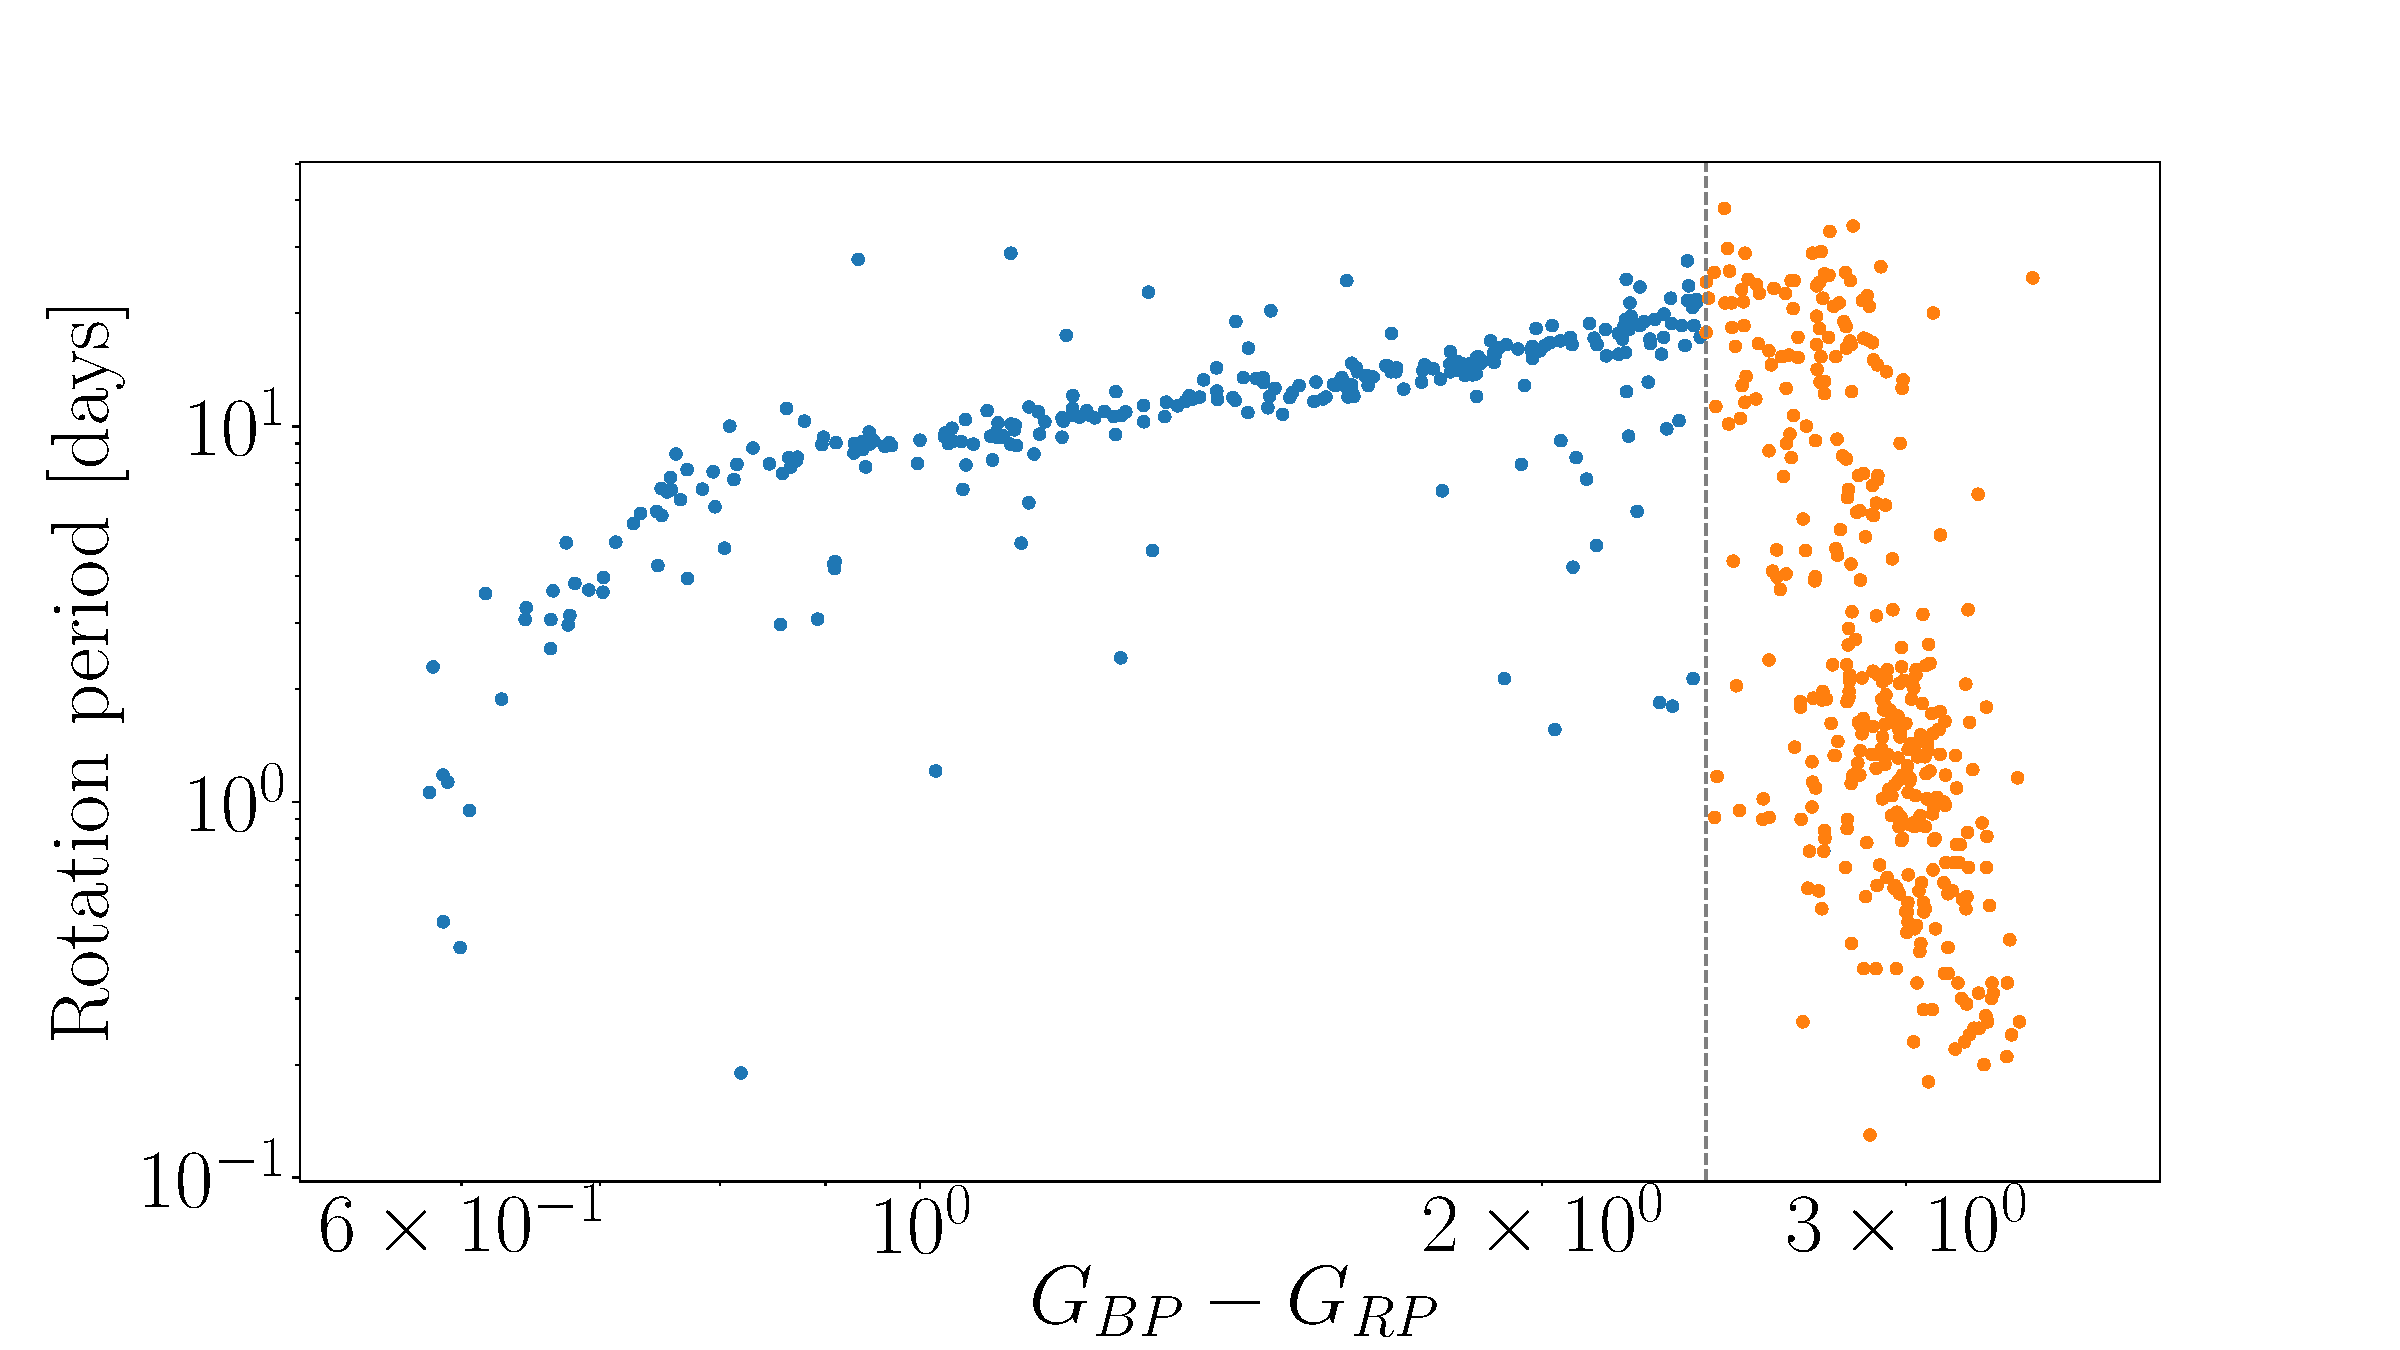
\includegraphics[width=1\textwidth]{praesepe.pdf}
% \label{fig:metallicity}
 % \end{figure}


% \section{Discussion}
% \label{section:discussion}
% Implications
%-----------------------------------------------------------------------------
%   - Summarize the results
%   - How including the rotation period improves precision of all parameters.
%   - How will this be used/what will it be useful for?
%   - Where is it not useful?

% Future and improvements
%-----------------------------------------------------------------------------
%   - A more sophisticated gyrochronology model
%   - Mixture model, etc.

% Rolling out/future
%   - Adding new datasets/dimensions/methods.
%-----------------------------------------------------------------------------

% What if you don't have a rotation period?
% Future surveys
\section{Discussion}
\label{section:discussion}

In the previous sections we demonstrated that modeling the ages of stars using
isochrones {\it and} gyrochronology can result in more precise ages than using
isochrone fitting alone.
Isochrone fitting and gyrochronology are  complementary because gyrochronology
is more precise where isochrone fitting is less precise (on the MS) and vice
versa (at MS turn off).
% Age precision is determined by the spacing of isochrones or gyrochrones: in
% regions where iso/gyrochrones are more tightly spaced, ages will be less
% precise.
% Isochrones becone less tightly spaced (and more precise) at larger stellar
% masses and lower surface gravities.
% Gyrochrones become more tightly spaced (and less precise) at larger stellar
% masses.
%   - How will this be used/what will it be useful for?
The method we present here is available as a {\it python} package called \sd\
which allows users to infer ages from their available apparent magnitudes,
parallaxes, rotation periods and spectroscopic propertes in just a few lines
of code.
This method is applicable to an extremely large number of stars: late F, GK
and early M stars with a rotation period and broad-band photometry.
This already includes tens-of-thousands of \kepler\ and \ktwo\ stars and could
include millions more from \tess, \lsst, \wfirst, \plato, \gaia, and others in
future.
Although this method is designed for combining isochrone fitting with
gyrochronology, \sd\ can still be used without rotation periods, in
which case it will predict an isochrone-only stellar age.
% \sd\ is therefore applicable to all stars covered by the MIST isochrones:
% masses from 0.1 to 300 M$_\odot$, ages ranging from 100,000 years to longer
% than the age of the Universe, and metallicities from -4 to 0.5.
However, it is {\it optimally applicable} to stars with rotation periods,
otherwise the result will be identical to ages measured with {\tt
isochrones.py}.
%   - Where is it not useful?
However, \sd\ will often predict inaccurate ages for stars younger than around
500 million years, where stars are more likely to be rapidly rotating
outliers, and close binaries whose interactions influence their rotation
period evolution.
% These ages may still be precise even though they are inaccurate.
% Building a mixture model into \sd\ would allow these outliers to be identified
% and this is one of the main improvements to \sd\ that we plan to make in
% future.
% Since many stars with measurable rotation periods do not have precise
% spectroscopic properties, it is not always possible to tell whether a star
% falls within these permissable ranges of masses, surface gravities and rossby
% numbers.
% In addition, any given star, even if it does meet the criteria for mass,
% age, binarity, etc, may still be a rotational outlier.
Rotational outliers are often seen in clusters \citep[see \eg][]{douglas2016,
rebull2016, douglas2017, rebull2017} and many of these fall above the main
sequence, indicating that they are binaries.
When a star's age is not accurately represented by its rotation period, its
isochronal age will be in tension with its gyrochronal one, however, given the
high information content of gyrochronology, the gyrochronal age will dominate
on the MS.
% Figure \ref{fig:bimodal} shows the posterior PDF for a star with a
% misrepresentative rotation period.
% This star is rotating more rapidly than its age and mass indicate it should,
% so the gyrochronal age of this star is under-predicted.
% Situations like this are likely to arise relatively often, partly because
% rotational spin-down is not a perfect process and some unknown physical
% processes can produce outliers, and partly because misclassified giants, hot
% stars, M dwarfs or very young or very old stars will not have rotation periods
% that relate to their ages in the same way.
In addition, measured rotation periods may not always be accurate and can, in
many cases, be a harmonic of the true rotation period.
A common rotation period measurement failure mode is to measure half the true
rotation period.
The best way to prevent an erroneous or outlying rotation period from
resulting in an erroneous age measurement is to {\it allow} for outlying
rotation periods using a mixture model.
We intend to build a mixture model into \sd\ in future.
% As shown in figure \ref{fig:praesepe}, the gyrochronology model used here
% \citep{angus2015} does not provide a good fit to all available data.
% In future we intend to calibrate a new gyrochronology model that fits all
% available cluster and asteroseismic data.
% For now however, we simply warn users of these caveats and suggest that ages
% calculated using \sd\ are treated with appropriate caution.

% %   - Caveats and gotchas -- e.g. isochrones aren't 100% accurate.
% Throughout this manuscript we have referred to the `accuracy' of the
% isochronal models.
% In reality though, stellar evolution models are not 100\% accurate and
% different stellar evolution models, \eg, MIST, Dartmouth, Yonsei-Yale, etc
% will predict slightly different ages.
% The disagreement between these models varies with position on the HRD,
% but in general, ages predicted using different stellar evolution models will
% vary by around 10\%.
% We use the MIST models in our code because they cover a broader range of ages,
% masses and metallicities than the Dartmouth models.

% %   - How including the rotation period improves precision of all parameters.
% Our focus so far has been on stellar age because this is the most difficult
% stellar parameter to measure.
% However, if the age precision is improved, then the mass, \feh, distance and
% extinction precision must also be improved, since these parameters are
% strongly correlated and co-dependent in the isochronal model.
% Figure \ref{fig:mass_improvement} shows the improvement in relative precision
% of mass measurements from our simulated star sample.


% Conclusion
% \label{section:conclusion}
% Summarize. the. paper.
%-----------------------------------------------------------------------------
%   - The model
%   - The tests
%   - The results
%   - The discussion
%   - The future
\section{Conclusion}
\label{section:conclusion}

We present a statistical framework for measuring precise ages of MS stars and
subgiants by combining observables that relate, via different evolutionary
processes, to stellar age.
Specifically, we combined HRD/CMD placement with rotation periods, in a
hierarchical Bayesian model, to age-date stars based on both their hydrogen
burning and magnetic braking history.
The two methods of isochrone fitting and gyrochronology were combined by
taking the product of two likelihoods: one that contains an isochronal model
and the other a gyrochronal one.
We used the MIST stellar evolution models and computed isochronal ages and
likelihoods using the {\tt isochrones.py} {\it Python} package.
We fit a new broken power law gyrochronology model to the Praesepe cluster
and included a modification recommended by \citet{vansaders2016} that accounts
for weakened magnetic braking at Rossby numbers larger than 2.
The rotation periods of hot stars, cool stars, evolved stars, young stars and
extremely metal poor and rich stars were modeled stochastically with a broad
log-normal distribution.
We tested \sd\ on simulated data and cluster stars and demonstrated that
combining gyrochronology with isochrone fitting increases the precision of age
estimates, compared to using isochrone fitting alone.

\sd\ may predict inaccurate ages for stars in close binaries whose
interactions influence their rotation period evolution.
Rotational outliers are often seen in clusters \citep[see \eg][]{douglas2016,
rebull2016, douglas2017, rebull2017} and many of these fall above the main
sequence on a CMD, indicating that they are binaries.
In addition, measured rotation periods may not always be accurate and can, in
many cases, be a harmonic of the true rotation period.
For example, a common rotation period measurement failure mode is to measure
half the true rotation period.
The best way to prevent an erroneous or outlying rotation period from
resulting in an erroneous age measurement is to {\it allow} for outlying
rotation periods using a mixture model, and we intend to build a mixture model
into \sd\ in future.

% Motivation
The optimal way to age-date stars is by combining {\it all} their available
age-related observables.
This could ultimately include activity dating via flare rates and
chromospheric activity indices, kinematic dating and chemical dating.
Of all the established age-dating methods, gyrochronology and isochrone
fitting are two of the most complementary.
The two methods are optimal in different parts of the HRD:
gyrochronology works well for FGK dwarfs and isochrone fitting works well for
subgiants and hot stars, so combining the two methods results in consistently
precise ages across a range of masses, ages and evolutionary stages.
In addition, using both methods at once circumvents the need to decide which
method to use {\it a priori}.
It eliminates the circular process of classifying a star based on its CMD
position (M dwarf, subgiant, etc), then deciding which age-dating method to
use, then inferring an age which itself depends on the classification that was
made.
It is important to infer all stellar properties at once since they all depend
on each other.
\sd\ is applicable to a large number of stars: AFGKM dwarfs and subgiants with
a rotation period and broad-band photometry.
This already includes tens-of-thousands of \kepler\ and \ktwo\ stars and could
include millions more from \tess, \lsst, \wfirst, \plato, \gaia, and others in
future.

The code used in this project is available as a {\it python} package called
\sd.
It is available for download via Github\footnote{git clone
https://github.com/RuthAngus/stardate.git} or through
PyPI\footnote{pip install stardate\_code}.
Documentation is available at https://stardate.readthedocs.io/en/latest/.
All code used to produce the figures in this paper is available at
https://github.com/RuthAngus/stardate.
\racomment{add github hash and Zenodo doi}.


% \section{Appendix}
% \label{section:appendix}
\section{Appendix}
\label{section:appendix}

\subsection*{Priors}
\label{section:priors}

We used the default priors in the {\tt isochrones.py} {\it python} package.
The prior over age was,
\begin{equation}
p(A) = \frac{\log(10) 10^{A}}{10^{10.5} - 10^8}, ~~~ 8 < A < 10.5.
\end{equation}
% where $A$, is $\log_{10}(\frac{\mathrm{Age}}{\mathrm{yrs}})$.
where $A$, is $\log_{10}(\mathrm{Age~[yrs]})$.
% The prior over mass is uniform in natural-log between -20 and 20,
% \begin{equation}
%     p(M) = U(-20, 20)
% \end{equation}
% % where $M$ is $\ln(\frac{\mathrm{mass}}{M_\odot})$.
% where $M$ is $\ln(\mathrm{Mass}~[M_\odot])$.
The prior over EEP was uniform with an upper limit of 800.
We found that adding this upper limit reduced some multi-modality caused by
the giant branch and resulted in better performance.
The prior over true bulk metallicity was based on the galactic metallicity
distribution, as inferred using data from the Sloan Digital Sky Survey
\citep{casagrande2011}.
% It is based on two double-Gaussian distribution, where the halo is described as
% a broad Gaussian and the galactic disc as a narrow Gaussian.
It is the product of a Gaussian that describes the metallicity distribution
over halo stars and two Gaussians that describe the metallicity distribution
in the thin and thick disks:
\begin{eqnarray}
    p(F) =
    & H_F \frac{1}{\sqrt{2\pi\sigma_{\mathrm{halo}}^2}}
    \exp\left(-\frac{(F-\mu_{\mathrm{halo}})^2}{2\sigma_{\mathrm{halo}}}\right)
    \\ \nonumber
    & \times (1-H_F)
    \frac{1}{\xi}
    \left[\frac{0.8}{0.15}\exp\left(-\frac{(F-0.016)^2}{2\times 0.15^2}\right)
    + \frac{0.2}{0.22}\exp\left(-\frac{(F-0.15)^2}{2\times
    0.22^2}\right)\right],
\end{eqnarray}
where $H_F = 0.001$ is the halo fraction, $\mu_\mathrm{halo}$ and
$\sigma_{\mathrm{halo}}$ are the mean and standard deviation of a Gaussian
that describes a probability distribution over metallicity in the halo, and
take values -1.5 and 0.4 respectively.
% $\mu_\mathrm{disk, 1}$, $\mu_\mathrm{disk, 2}$, $\sigma_\mathrm{disk, 1}$
% and $\sigma_\mathrm{disk, 2}$ are the means and standard deviations of two
The two Gaussians inside the square brackets describe probability
distributions over metallicity in the thin and thick disks.
The values of the means and standard deviations in these Gaussians are from
\citet{casagrande2011}.
$\xi$ is the integral of everything in the square brackets from $-\infty$ to
$\infty$ and takes the value $\sim 2.507$.
% D_F = 0.8 \sigma_{\mathrm{disk, 1}} = 0.15 \mu_{\mathrm{disk, 1}} = 0.016
% \sigma_{\mathrm{disk, 2}} = 0.22 \mu_{\mathrm{disk, 2}} = 0.15
The prior over distance was,
\begin{equation}
    p(D) = \frac{3}{3000^3} D^2, ~~~ 0 < D < 3000,
\end{equation}
with D in kiloparsecs, and, finally, the prior over extinction was uniform
between zero and one,
\begin{equation}
    p(A_V) = U(0, 1).
\end{equation}


% acknowledgements
Some of the data presented in this paper were obtained from the Mikulski
Archive for Space Telescopes (MAST).
STScI is operated by the Association of Universities for Research in
Astronomy, Inc., under NASA contract NAS5-26555.
Support for MAST for non-HST data is provided by the NASA Office of Space
Science via grant NNX09AF08G and by other grants and contracts.
This paper includes data collected by the Kepler mission. Funding for the
Kepler mission is provided by the NASA Science Mission directorate.

\bibliographystyle{plainnat}
\bibliography{hz.bib}
\end{document}
